\chapter{Аналитическая геометрия}
\section{Элементы векторной алгебры}
\subsection{Основные определения}
\(V\) --- пространство геометрических векторов.

Геометрический (свободный) вектор \(\vec a\) --- направленный отрезок в пространстве.

Длина (модуль) вектора \(|\vec a| = |\overrightarrow{AB}| = AB\) --- длина отрезка, на котором строится вектор.

Нулевой вектор \(\vec 0\) --- имеет длину ноль, начало совпадает с концом.

Вектор независим от точки приложения (его начала)

\(\vec a \parallel \vec b \defLeftrightarrow\) они лежат на одной или параллельных прямых \(\defLeftrightarrow\vec a,\vec b\) коллинеарны.

\(\forall \vec a:\vec 0 \parallel \vec a\)

\(\upuparrows\) и \(\updownarrows\) --- обозначение сонаправленности и разнонаправленности векторов.

\(
\vec a = \vec b\ \defLeftrightarrow
\begin{cases*}
    \vec a \upuparrows \vec b \\
    |\vec a| = |\vec b|       \\
\end{cases*}
\)

\(\vec a, \vec b, \vec c\) - компланарны \(\defLeftrightarrow\) лежат или параллельны одной плоскости.

\(\vec a_0\) --- орт вектор вектора \(\vec a \defLeftrightarrow\)
\(
\begin{cases*}
    \vec a_0 \upuparrows \vec a \\
    |\vec a_0| = 1              \\
\end{cases*}
\)

Вектора можно складывать: \(\vec a + \vec b = \vec c\). Строится по правилу треугольника или параллелограмма.

Вектора можно умножать на скаляр: \(\vec c = \vec a \cdot \lambda, \lambda \in \mathbb R\).
\begin{itemize}
    \item[] \(|\vec c| = |\vec a| \cdot |\lambda|\)
    \item[] \(\lambda > 0: \vec a \upuparrows \vec c\)
    \item[] \(\lambda < 0: \vec a \updownarrows \vec c\)
    \item[] \(\lambda = 0: \vec c = \vec 0\)
\end{itemize}
Вектора можно вычитать: \(\vec a - \vec b = \vec a + (-1) \cdot \vec b = \vec c\).

У \((V, ``+" \,, ``\cdot \lambda")\) есть свойства:
\begin{enumerate}
    \item \(\forall \vec a, \vec b: \vec a + \vec b = \vec b + \vec a\)
    \item \(\forall \vec a, \vec b, \vec c: (\vec a + \vec b) + \vec c = \vec a + (\vec b + \vec c)\)
    \item \(\exists \vec 0: \forall \vec a: \vec a + \vec0 = \vec a\)
    \item \(\forall \vec a: \exists (- \vec a): \vec a+(- \vec a) = \vec 0\)
    \item \(\forall \lambda \in \mathbb R: \forall \vec a, \vec b: \lambda (\vec a + \vec b) = \lambda \vec a + \lambda \vec b\)
    \item \(\forall \lambda, \mu \in \mathbb R: \forall \vec a: (\lambda + \mu)\vec a = \lambda \vec a + \mu \vec a\)
    \item \(\forall \lambda, \mu \in \mathbb R: \forall \vec a: (\lambda \mu)\vec a = \mu(\lambda \vec a) = \lambda (\mu \vec a )\)
    \item \(\forall \vec a: 1 \cdot \vec a = \vec a\)
\end{enumerate}

Вcё это доказывается из школьной геометрии. Эти свойства (аксиомы) линейного пространства \(\Rightarrow (V, ``+" \,, ``\cdot \lambda")\) --- линейное пространство.

\(
\vec v_1, \vec v_2, \dots, \vec v_n \in V , 
    \lambda_1, \lambda_2, \dots, \lambda_n \in \mathbb{R}
\Rightarrow \sum\limits_{i = 1}^{n} \lambda_i \vec v_i = \vec v\) --- линейная комбинация векторов \(\vec v_1, \vec v_2, \dots, \vec v_n\), или \(\vec v\) разложен по векторам \(\vec v_1, \vec v_2, \dots, \vec v_n\).

\(\sum\limits_{i = 1}^{n} \lambda_i \vec v_i = \vec 0\) --- нулевая линейная комбинация.

Линейная комбинация --- тривиальная \(\defLeftrightarrow \forall i \in \{1, \dots, n\}: \lambda_i = 0\)

Система векторов \(\vec v_1, \vec v_2, \dots, \vec v_n\) --- линейно независимая \(\defLeftrightarrow\) все её нулевые линейные комбинации --- тривиальные. То есть система векторов \(\vec v_1, \vec v_2, \dots, \vec v_n\) --- линейно независимая \(\defLeftrightarrow \sum\limits_{i = 1}^{n} \lambda_i \vec v_i = \vec 0 \Leftrightarrow \forall i \in \{1, \dots, n\}: \lambda_i = 0\). Пример: \(\forall a, b : a \nparallel b \Leftrightarrow \vec a, \vec b\) - линейно-независимы

Система векторов \(\vec v_1, \vec v_2, \dots, \vec v_n\) --- линейно зависимая \(\defLeftrightarrow\) существует её нулевая нетривиальная линейная комбинация. То есть система векторов \(\vec v_1, \vec v_2, \dots, \vec v_n\) --- линейно зависимая \(\defLeftrightarrow \exists \lambda_i \neq 0:\sum\limits_{i = 1}^{n} \lambda_i \vec v_i = \vec 0\). Пример: \(\forall a, b : a \parallel b\Leftrightarrow \vec a, \vec b\) - линейно-зависимы

Свойства линейной зависимости:
\begin{enumerate}
    \item \(\vec 0 \in \{\vec v_1, \vec v_2, \dots, \vec v_n\} \Rightarrow \vec v_1, \vec v_2, \dots, \vec v_n\) --- линейно зависимая система.

          Пусть \(\vec v_k = \vec 0\). Возьмём \(\lambda_k = 1\), а \(\forall i \neq k: \lambda_i = 0\). Значит \(\sum\limits_{i = 1}^{n} \lambda_i \vec v_i = 0 \vec v_1 + 0 \vec v_2 + \dots + 1 \vec v_k + \dots + 0 \vec v_n = 1 \cdot \vec 0 = \vec 0 \quad Q.E.D\)

    \item \(\vec v_1, \vec v_2, \dots, \vec v_n\) --- линейно зависимая система \(\Rightarrow \vec v_1, \vec v_2, \dots, \vec v_n, \vec v_{n + 1}, \vec v_{n + 2}, \dots \vec v_{n + m}\) --- линейно зависимая система.

          Возьмём \(\lambda_1, \lambda_2, \dots, \lambda_n\), создающие нулевую нетривиальную линейную комбинацию, а \(\forall i \in \{n + 1, n + 2, \dots, n + m\}\) возьмём \(\lambda_i = 0\). Тогда \(\sum\limits_{i = 1}^{n + m} \lambda_i \vec v_i = \sum\limits_{i = 1}^{n} \lambda_i \vec v_i = 0 \vec v_{n + 1} + 0 \vec v_{n + 2} + \dots + 0 \vec v_{n + m} = \vec 0 + \vec 0 = \vec 0 \quad Q.E.D\)\\

    \item В линейно зависимой системе \(\vec v_1, \vec v_2, \dots, \vec v_n\) есть вектор, который можно выразить линейной комбинацией других, то есть \(\exists \vec v_k: v_k = \sum\limits_{i = 1, i \neq k}^{n} \mu_i \vec v_i\).

          Возьмём \(\lambda_1, \lambda_2, \dots, \lambda_n\), создающие нулевую нетривиальную линейную комбинацию \(\Rightarrow \exists \lambda_k \neq 0 \Rightarrow \lambda_k \vec v_k = \sum\limits_{i = 1, i \neq k}^{n} \lambda_i \vec v_i \Rightarrow\) возьмём \(\mu_i = \frac{\lambda_i}{\lambda_k} \Rightarrow v_k = \sum\limits_{i = 1, i \neq k}^{n} \mu_i \vec v_i \quad Q.E.D\)

\end{enumerate}

Базис прямой --- любой ненулевой вектор на этой прямой.

\deff{def:} Базис плоскости --- любая упорядоченная пара неколлинеарных векторов в данной плоскости.
Базис пространства --- любая упорядоченная тройка некомпланарных векторов в этом пространстве.

\(\vec e_1, \vec e_2, \vec e_3\) --- базис пространства.

\deff{def:} \(\vec x = \sum\limits_{i = 1}^{3} \vec e_i x_i, x_i \in \mathbb{R} \Rightarrow (x_1, x_2, x_3)\) --- координаты \(\vec x\) относительно базиса \(\vec e_1, \vec e_2, \vec e_3\). Аналогично для плоскости и прямой.

\begin{enumerate}
    \item \(\forall \vec x \parallel L \; \exists! x_1 \in \mathbb{R}: \vec x = x_1 \vec e_1\), где \(\vec e_1\) --- базис прямой \(L\).

          Пусть \(O \in L\). Приложим к \(O\) начала векторов \(\vec x\) и \(\vec e_1\). \(\vec x_1 \parallel \vec e_1 \Leftrightarrow \exists! x \in \mathbb{R}: \vec x = x_1 \vec e_1\) \(Q.E.D.\)  
               \[\vec e_1 \upuparrows \vec x: x_1 > 0\]
               \[\vec e_1 \updownarrows \vec x: x_1 < 0\]
              \[\vec x = \vec 0: x_1 = 0\]
    \item \(\forall \vec x \parallel \alpha \; \exists! x_1, x_2 \in \mathbb{R}: \vec x = x_1 \vec e_1 + x_2 \vec e_2\), где \(\vec e_1, \vec e_2\) --- базис плоскости \(\alpha\).

          Аналогично, пусть \(O \in \alpha\). Приложим к \(O\) начала векторов \(\vec x, \vec e_1\) и \(\vec e_2\). 

          \begin{enumerate}
              \item   \(\vec x = \vec 0: \vec x = 0 \vec e_1 + 0 \vec e_2\). 
              \item  \(\vec x \neq \vec 0:\) пусть \(B\) --- конец \(\vec x\). Проведём \(L_2 \parallel \vec e_2, B \in L_2\).

          Проведём \(L_1 \parallel \vec e_1, O \in L_1\). \(A = L_1 \cap L_2\). \(\vec x = \overrightarrow{OB} = \overrightarrow{OA} + \overrightarrow{AB}\).

          \(
          \begin{rcases*}
              \overrightarrow{OA} \parallel \vec e_1 \Rightarrow (\text{по пункту 1}) \Rightarrow \exists! x_1 \in \mathbb{R}: \overrightarrow{OA} = x_1 \vec e_1 \\
              \overrightarrow{AB} \parallel \vec e_2 \Rightarrow (\text{по пункту 1}) \Rightarrow \exists! x_2 \in \mathbb{R}: \overrightarrow{AB} = x_2 \vec e_2
          \end{rcases*}
          \Rightarrow \vec x = x_1 \vec e_1 + x_2 \vec e_2\) \(Q.E.D.\)
          \end{enumerate}
         

         

    \item \(\forall \vec x \in V \; \exists! x_1, x_2, x_3 \in \mathbb{R}: \vec x = x_1 \vec e_1 + x_2 \vec e_2 + x_3 \vec e_3\), где \(\vec e_1, \vec e_2, \vec e_3\) --- базис \(V\).

          Пусть \(O \in V\). Приложим к \(O\) начала векторов \(\vec x, \vec e_1, \vec e_2\) и \(\vec e_3\). \(\alpha(O, \vec e_1, \vec e_2)\). 

          \begin{enumerate}
              \item  \(\vec x = \vec 0: \vec x = 0 \vec e_1 + 0 \vec e_2 + 0 \vec e_3\).
              \item  \(\vec x \neq \vec 0:\) пусть \(B\) --- конец \(\vec x\). Проведём \(L \parallel \vec e_3, B \in L\). \(A = L \cap \alpha\). \(\vec x = \overrightarrow{OB} = \overrightarrow{OA} + \overrightarrow{AB}\).

          \(
          \begin{rcases*}
              \overrightarrow{OA} \parallel \vec \alpha \Rightarrow (\text{по пункту 2}) \Rightarrow \exists! x_1, x_2 \in \mathbb{R}: \overrightarrow{OA} = x_1 \vec e_1 + x_2 \vec e_2 \\
              \overrightarrow{AB} \parallel \vec e_3 \Rightarrow (\text{по пункту 1}) \Rightarrow \exists! x_3 \in \mathbb{R}: \overrightarrow{AB} = x_3 \vec e_3
          \end{rcases*}
          \Rightarrow \vec x = x_1 \vec e_1 + x_2 \vec e_2 + x_3 \vec e_3\) 
          \end{enumerate}
           \hfill Q.E.D
\end{enumerate}

То есть, любой вектор может быть разложен по базису, и единственным образом.

Следствия:
\begin{enumerate}
    \item \(\vec a = \sum\limits_{i = 1}^{3} a_i \vec e_i, \vec b = \sum\limits_{i = 1}^{3} b_i \vec e_i: \vec a = \vec b \Leftrightarrow \forall i \in \{1, 2, 3\}: a_i = b_i\)

    \item \(\vec a + \vec b = \vec c = \sum\limits_{i = 1}^{3} c_i \vec e_i \Leftrightarrow \forall i \in \{1, 2, 3\}: c_i = a_i + b_i\)

          \(\vec c = \vec a + \vec b = \sum\limits_{i = 1}^{3} a_i \vec e_i + \sum\limits_{i = 1}^{3} b_i \vec e_i = \sum\limits_{i = 1}^{3} (a_i + b_i) \vec e_i = \sum\limits_{i = 1}^{3} c_i \vec e_i \Leftrightarrow \forall i \in \{1, 2, 3\}: c_i = a_i + b_i\) \(Q.E.D.\)

    \item \(\lambda \vec a = \vec c = \sum\limits_{i = 1}^{3} c_i \vec e_i \Leftrightarrow \forall i \in \{1, 2, 3\}: c_i = \lambda a_i\)

          \(\vec c = \lambda \vec a = \lambda \sum\limits_{i = 1}^{3} a_i \vec e_i = \sum\limits_{i = 1}^{3} (\lambda a_i) \vec e_i = \sum\limits_{i = 1}^{3} c_i \vec e_i \Leftrightarrow \forall i \in \{1, 2, 3\}: c_i = \lambda a_i\) 

\hfill Q.E.D
\end{enumerate}

\(\vec a \parallel \vec b \Leftrightarrow \exists \lambda \in \mathbb{R}:
\left[
\begin{array}{ll}
    \vec a = \lambda \vec b \\
    \vec b = \lambda \vec a
\end{array}
\right .
\Leftrightarrow
\forall i \in \{1, 2, 3\}:
\left[
\begin{array}{ll}
    a_i = \lambda b_i \\
    b_i = \lambda a_i
\end{array}
\right .
\Leftrightarrow \frac{a_1}{b_1} = \frac{a_2}{b_2} = \frac{a_3}{b_3} = \lambda\) --- коэффициент пропорциональности.

\(\vec v_1, \vec v_2, \vec v_3, \dots, \vec v_n\) --- коллинеарны \(\Rightarrow\) они линейно зависимы в пространстве.

\newpage

\subsection{Система координат на плоскости и в пространстве}

Говорят, что в пространстве введена декартова система координат (ДСК), если зафиксирована \((\cdot) O \)(начало координат) и базис \(\vec{e}_1, \vec{e}_2, \vec{e}_3\)

Оси координат --- прямые, содержащие базисные вектора, приложенные к точке O.

\(Ox\) - абсцисс, \(Oy\) - ординат, \(Oz\) - аппликат

 \begin{center}
    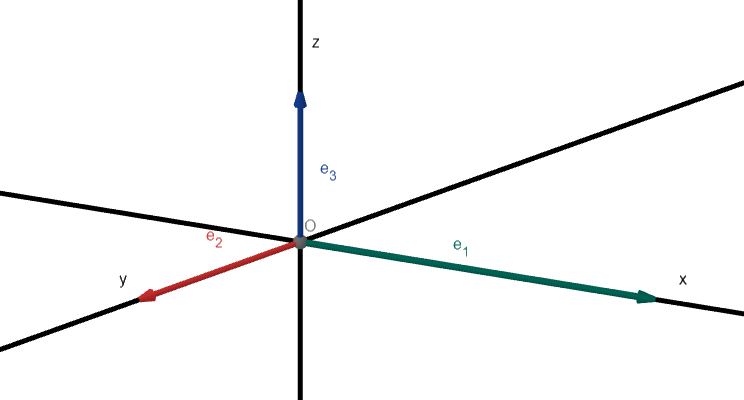
\includegraphics[height=6cm]{Images/Chapter_1/1-2-3.png}
 \end{center}

Координатами точки \(M\) в ДСК \((O, \vec{e_1}, \vec{e_2}, \vec{e_3})\) называются координаты вектора \(\overrightarrow{OM}\) в базисе \((\vec{e_1}, \vec{e_2}, \vec{e_3})\). 

Если вам даны 2 точки: \(A(a_1, a_2, a_3), B(b_1, b_2, b_3)\),то \(\overrightarrow{AB} = (b_1-a_1,b_2-a_2,b_3-a_3)\), т.к. \(\overrightarrow{AB}= \overrightarrow{OB} - \overrightarrow{OA}\) 

Задача: Даны 2 точки: \(A(a_1, a_2, a_3), B(b_1, b_2, b_3)\) и точка \(M = (m_1, m_2, m_3)\), делящая отрезок AB в отношении \(\frac{AM}{MB}=\lambda > 0\). Найти координаты точки \(M\) через \(A, B, \lambda\).
\[AM = \lambda MB \Leftrightarrow |\overrightarrow{AM}| = \lambda |\overrightarrow{MB}| \Rightarrow \overrightarrow{AM} = \lambda \overrightarrow{MB}\]
\[\forall i=1,2,3:m_i - a_i = \lambda (b_i - m_i) \Leftrightarrow m_i = \frac{\lambda b_i + a_i}{1 + \lambda}\]
Откуда координаты точки $M$ найдены и задача решена.

В дальнейшем будем работать с ортогональной д.с.к., где \(\vec{e_1},\vec{e_2},\vec{e_3}\) попарно ортоганальны и нормированы \((|e_i|=1)\).

Длина вектора в ортонормированной декартовой системе координат равна квадратному корню суммы квадратов координат:
\[|\vec a| = \sqrt{\sum\limits_{i=1}^3a_i^2}\]
\(\vec a = \sum\limits_{i=1}^3 a_i \vec e _i\) - разложение по координатам.

\(\overrightarrow{a_0} = \cfrac{\vec a}{|\vec a|}\) - называется ортом, причем $\overrightarrow{a_0} = (\cos \alpha, \cos \beta, \cos \gamma)$. 

Такие косинусы называются направляющими.

 \begin{center}
    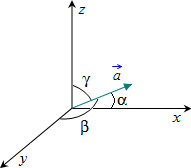
\includegraphics[height=4cm]{Images/Chapter_1/1-2-2.png}
 \end{center}
 
Причем $a_1 = |a| \cdot \cos \alpha$, $a_2 = |a| \cdot \cos \beta$, $a_3 = |a| \cdot \cos \gamma$

В трёхмерном пространстве сумма квадратов косинусов углов между радиус-вектором точки и осями координат равна единице:
\[\cos^2 \alpha  + \cos^2 \beta  + \cos^2 \gamma =1\]


Полярная система координат на плоскости --- это точка (начало системы координат $O$) и луч, исходящий из неё, на плоскости. При этом координатами точки до какой-либо точки $M$ являются длина $r =|\overrightarrow{OM}|$ и угол, который составляет вектор $\overrightarrow{OM}$ с выбранным лучом, равный $\varphi$. У точки ноль нет полярных координат, считают, что у нее \(r=0\).

\begin{center}
    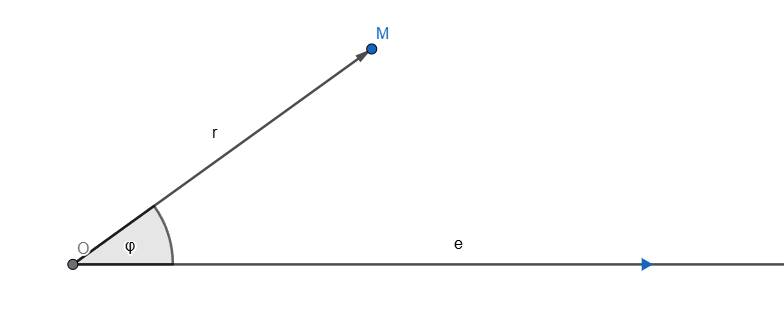
\includegraphics[height = 5.5cm]{Images/Chapter_1/1-2-4.png}
\end{center}
    
    

При этом выбор диапозона угла \(\varphi\) неоднозначен.

Связь между декартовыми и полярными координатами: Обычно ДСК связывают с ПСК так: центр общий, а полярный луч --- положительное направление \(Ox\). Тогда:
\[x=r\cos\varphi, y=r\sin\varphi\] 
Обратно: \[r=\sqrt{x^2 + y^2}, \varphi=\arctan\frac{y}{x} + \pi k\] (при этом выбор $k$ неоднозначен - зависит от диапазона и в какой четверти лежит точка)

\textbf{Пример:} Лемниската Бернулли

$(x^2+y^2)^2=x^2-y^2$. Но приведя в п.с.к:  \(r^4=r^2(\cos^2x-\sin^2x)\leftrightarrow r=\sqrt{\cos(2x)}\). В такой форме можно нарисовать эскиз графика:
\begin{center}
    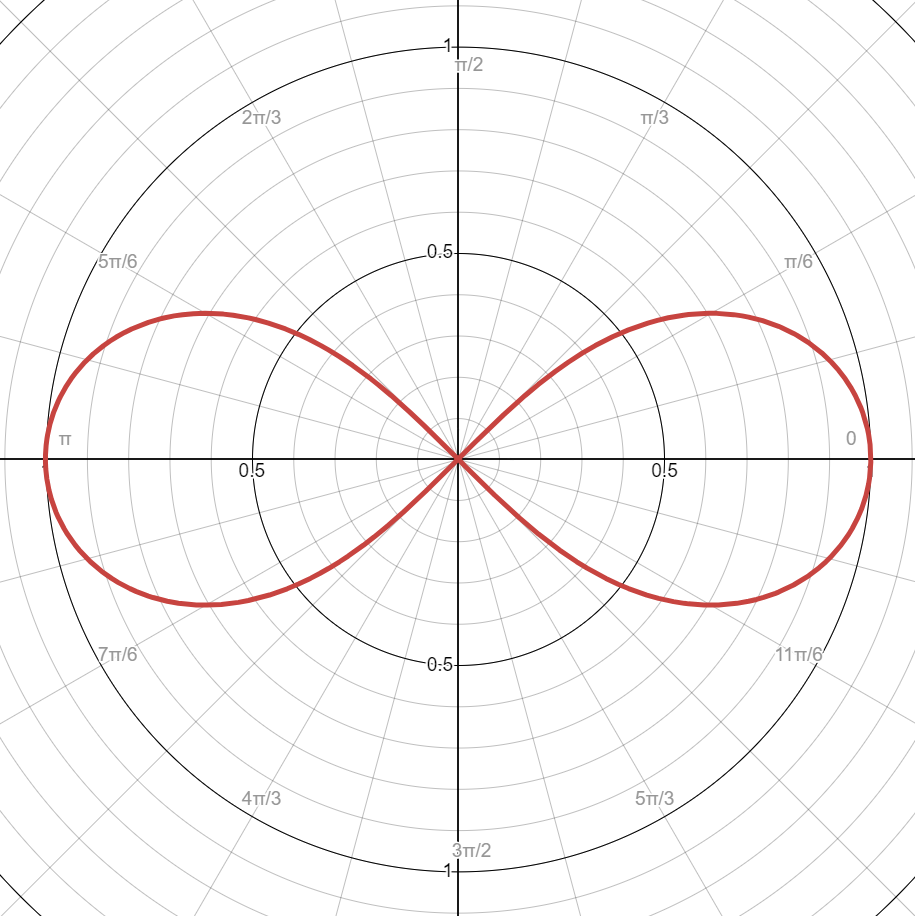
\includegraphics[height=12cm]{Images/Chapter_1/1-2-1.png}
\end{center}

\newpage

\subsection{Преобразования в ДСК}
\begin{enumerate}[label=\alph*)]
    \item Параллельный перенос
          \begin{center}
              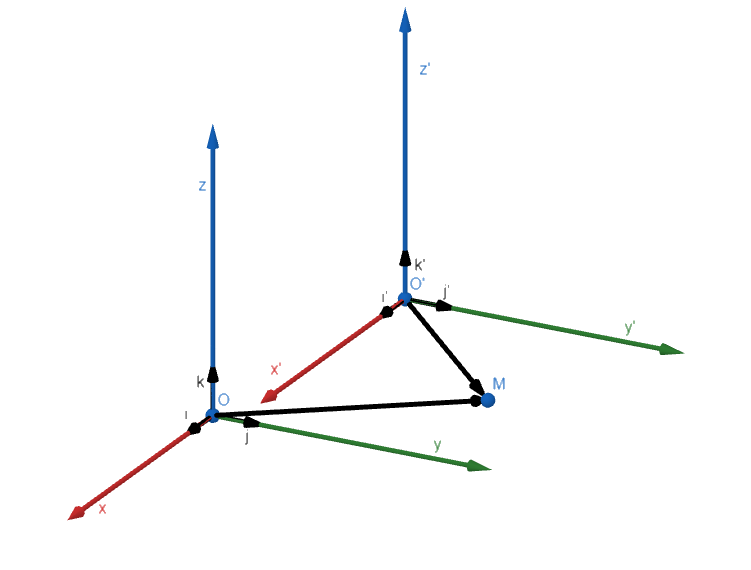
\includegraphics[height=7cm]{Images/Chapter_1/1-3-1.png}
          \end{center}
          Введем новую ДСК с центром в \(O' = (x_0, y_0, z_0)\). Заметим, что \(\overrightarrow{OM} = \overrightarrow{OO'} +  \overrightarrow{O'M}\). Тогда:

          \(M = (x, y, z) \text{(в старой)} = (x', y', z') \text{(в новой)} = (x_0 + x', y_0 + y', z_0 + z') \text{(в старой)}\)
    \item Поворот
          \begin{itemize}
              \item На плоскости:
                    \begin{center}
                        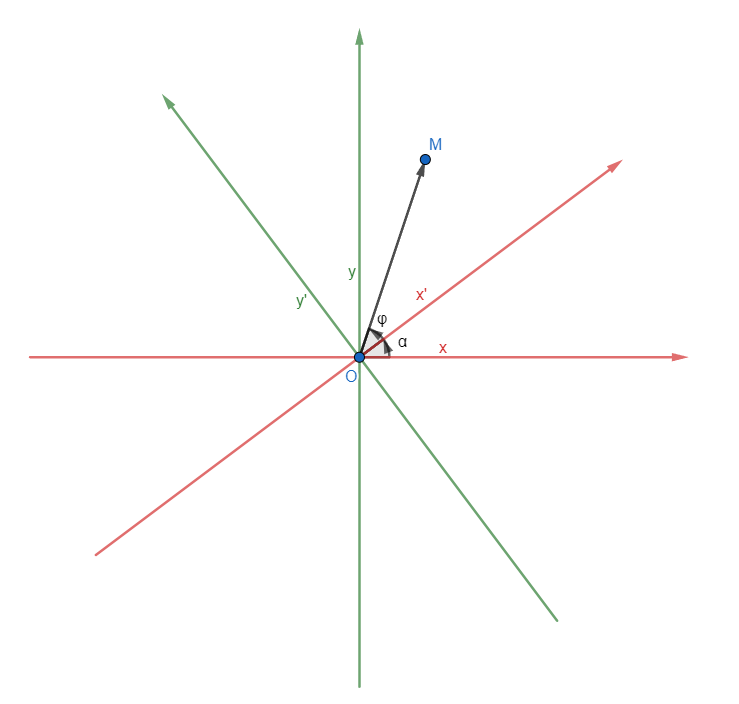
\includegraphics[height=7cm]{Images/Chapter_1/1-3-2.png}
                    \end{center}
                    Введем новую ДСК, повёрнутую на \(\alpha\). $(r,\varphi)$ п.с.к  в $Ox'y'$

                    \(M = (x, y) = (r \cos(\varphi + \alpha), r \sin(\varphi + \alpha)) =
                    (x' \cos\alpha - y' \sin\alpha, x' \sin\alpha + y' \cos\alpha)\)

                    \(\begin{pmatrix}
                        x \\
                        y
                    \end{pmatrix} =
                    \begin{pmatrix}
                        \cos\alpha & -\sin\alpha \\
                        \sin\alpha & \cos\alpha
                    \end{pmatrix}
                    \begin{pmatrix}
                        x' \\
                        y'
                    \end{pmatrix}\)

                    \(\begin{pmatrix}
                        x' \\
                        y'
                    \end{pmatrix} =
                    \begin{pmatrix}
                        \cos\alpha  & \sin\alpha \\
                        -\sin\alpha & \cos\alpha
                    \end{pmatrix}
                    \begin{pmatrix}
                        x \\
                        y
                    \end{pmatrix}\)

                    \(\begin{pmatrix}
                        \cos\alpha  & \sin\alpha \\
                        -\sin\alpha & \cos\alpha
                    \end{pmatrix}\) --- Матрица поворота.
              \item В пространстве:
                    \begin{center}
                        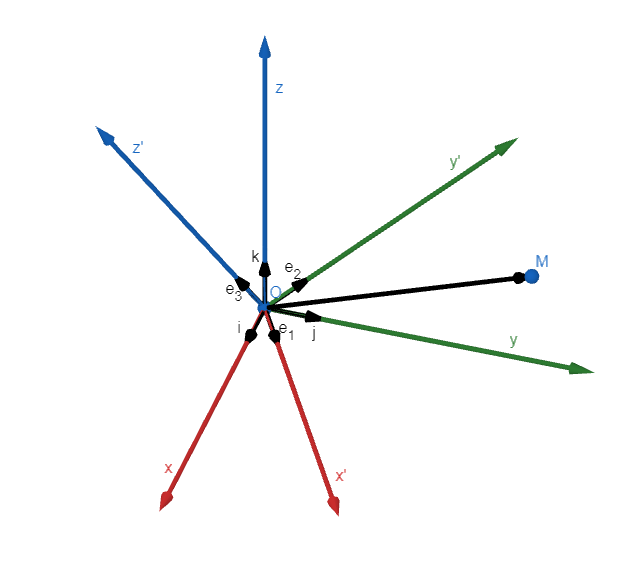
\includegraphics[height=7cm]{Images/Chapter_1/1-3-3.png}
                    \end{center}
                    Создадим новую ДСК, повёрнутую в пространстве.
                    Базис \(\vec i, \vec j, \vec k \rightarrow \vec e_1, \vec e_2, \vec e_3\).
                    Оси \(x, y, z \rightarrow x', y', z'\). Оба базиса попарно ортогональны и нормированы.

                    \(m = 1, 2, 3: \vec e_m = (\cos\alpha_m, \cos\beta_m, \cos\gamma_m)\) - направляющие косинусы.

                    \(M = (x, y, z) = x\vec i + y\vec j + z\vec k = \\
                    = x'(\cos\alpha_1\vec i + \cos\beta_1\vec j + \cos\gamma_1\vec k) + \\
                    + y'(\cos\alpha_2\vec i + \cos\beta_2\vec j + \cos\gamma_2\vec k) + \\
                    + z'(\cos\alpha_3\vec i + \cos\beta_3\vec j + \cos\gamma_3\vec k) = \\
                    = \vec i(x'\cos\alpha_1 + y'\cos\alpha_2 + z'\cos\alpha_3) + \\
                    + \vec j(x'\cos\beta_1 + y'\cos\beta_2 + z'\cos\beta_3) + \\
                    + \vec k(x'\cos\gamma_1 + y'\cos\gamma_2 + z'\cos\gamma_3)\)

                    Т.к. координаты точки задаются единственным способом, то:

                    \(\begin{cases*}
                        x = x'\cos\alpha_1 + y'\cos\alpha_2 + z'\cos\alpha_3 \\
                        y = x'\cos\beta_1 + y'\cos\beta_2 + z'\cos\beta_3    \\
                        z = x'\cos\gamma_1 + y'\cos\gamma_2 + z'\cos\gamma_3
                    \end{cases*}\)

                    \(\begin{pmatrix}
                        x \\
                        y \\
                        z
                    \end{pmatrix} =
                    \begin{pmatrix}
                        \cos\alpha_1 & \cos\alpha_2 & \cos\alpha_3 \\
                        \cos\beta_1  & \cos\beta_2  & \cos\beta_3  \\
                        \cos\gamma_1 & \cos\gamma_2 & \cos\gamma_3
                    \end{pmatrix}
                    \begin{pmatrix}
                        x' \\
                        y' \\
                        z'
                    \end{pmatrix}\)

                    Столбцы в этой матрице - координаты \(\vec e_1, \vec e_2, \vec e_3\).
          \end{itemize}
\end{enumerate}


\newpage
\subsection{Скалярное произведение векторов}

\(``\cdot": V_3 \times V_3 \rightarrow \mathbb{R}\)

\(\vec a, \vec b \in V_3 \rightarrow (\vec a, \vec b) = \vec a \cdot \vec b \in \mathbb{R}\)

\(\vec a \cdot \vec b = |\vec a| |\vec b| \cos\varphi;\; \varphi = \angle(\vec a, \vec b)\)
\begin{center}
    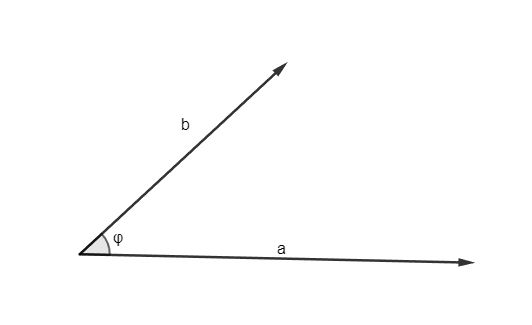
\includegraphics[height=7cm]{Images/Chapter_1/1-4-1.png}
\end{center}
Свойства: (\(\forall \vec a, \vec b \in V_3\))
\begin{enumerate}
    \item Симметричность: \(\vec a \cdot \vec b = \vec b \cdot \vec a\)

          Очевидно
    \item Аддитивность по 1-му аргументу: \(\forall \vec a_1, \vec a_2 \in V_3:
          (\vec a_1 + \vec a_2) \cdot \vec b = \vec a_1 \cdot \vec b + \vec a_2 \cdot \vec b\)

          \(\proj_{\vec b}\vec a\) --- Проекция \(\vec a\) на направление \(\vec b\).

          \(\proj_{\vec b}\vec a\ = |\vec a| \cos \varphi; \varphi = \angle(\vec a, \vec b) \in [0, \pi]\)

          \(\vec a = (a_x, a_y, a_z) \Rightarrow a_x = |\vec a| \cos\alpha;\; \alpha = \angle(\vec a, \vec i)\)
          \begin{center}
              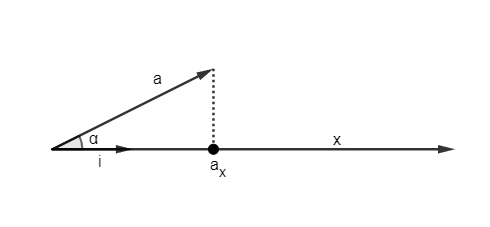
\includegraphics[height=7cm]{Images/Chapter_1/1-4-2.png}
          \end{center}
          \(a_x = \proj_{\vec i}\vec a = \vec i \cdot \vec a\),
          \(a_y = \proj_{\vec j}\vec a = \vec j \cdot \vec a\),
          \(a_z = \proj_{\vec k}\vec a = \vec k \cdot \vec a\)

          Выберем ДСК таким образом, что \(\vec i = \frac{\vec b}{|\vec b|}\) --- орт вектора \(\vec b\)
          \begin{center}
              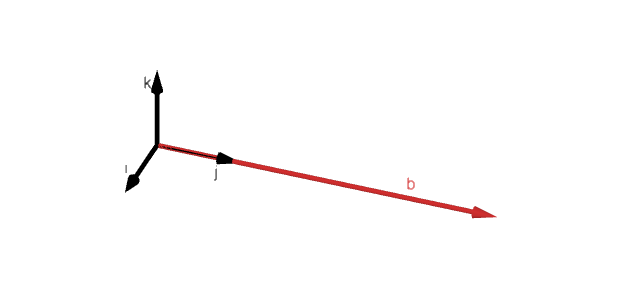
\includegraphics[height=7cm]{Images/Chapter_1/1-4-3.png}
          \end{center}
          \(\vec a = \vec a_1 + \vec a_2\)

          \((\vec a)_x = \proj_{\vec i}\vec a = \vec a \cdot \vec i =
          (\vec a_1 + \vec a_2) \cdot \frac{\vec b}{|\vec b|} =
          \frac{1}{|\vec b|} ((\vec a_1 + \vec a_2) \cdot \vec b)\)

          \(m = 1, 2: (\vec a_m)_x = \proj_{\vec i}\vec a_m = \vec a_m \cdot i =
          \vec a_m \cdot \frac{\vec b}{|\vec b|} =
          \frac{1}{|\vec b|} (\vec a_m \cdot \vec b)\)

          \(\begin{rcases*}
              \vec a = \frac{1}{|\vec b|} ((\vec a_1 + \vec a_2) \cdot \vec b) \\
              \vec a = \vec a_1 + \vec a_2 = \frac{1}{|\vec b|} (\vec a_1 \cdot \vec b) + \frac{1}{|\vec b|} (\vec a_2 \cdot \vec b)
          \end{rcases*} \Rightarrow \frac{1}{|\vec b|} ((\vec a_1 + \vec a_2) \cdot \vec b) =
          \frac{1}{|\vec b|} (\vec a_1 \cdot \vec b) + \frac{1}{|\vec b|} (\vec a_2 \cdot \vec b) \Rightarrow \\
          \Rightarrow (\vec a_1 + \vec a_2) \cdot \vec b = \vec a_1 \cdot \vec b + \vec a_2 \cdot \vec b \quad Q.E.D\)
    \item Однородность по 1-му аргументу: \(\forall \lambda \in \mathbb{R}: (\lambda \vec a)\cdot \vec b = \lambda(\vec a \cdot \vec b)\)
          \begin{center}
              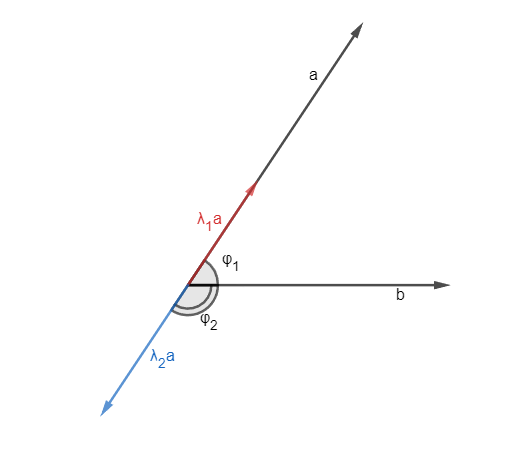
\includegraphics[height=7cm]{Images/Chapter_1/1-4-4.png}
          \end{center}
          \(|\lambda \vec a| = |\lambda| |\vec a|\)

          \(\lambda > 0: (\lambda \vec a)\cdot \vec b = |\lambda \vec a| |\vec b| \cos\varphi_1 = \lambda(|\vec a| |\vec b| \cos\varphi_1) = \lambda(\vec a \cdot \vec b)\)

          \(\lambda < 0: (\lambda \vec a)\cdot \vec b = |\lambda \vec a| |\vec b| \cos\varphi_2 = -\lambda(|\vec a| |\vec b| \cos\varphi_2) = \lambda(|\vec a| |\vec b| \cos(\pi - \varphi_2)) = \lambda(\vec a \cdot \vec b)\)

          \(\lambda = 0: (\lambda \vec a)\cdot \vec b = \vec 0 \cdot \vec b = 0 = 0(\vec a \cdot \vec b) = \lambda(\vec a \cdot \vec b)\)

          \(Q.E.D.\)
    \item \(\vec a \cdot \vec a \geq 0\). \(\vec a \cdot \vec a = 0 \Leftrightarrow \vec a = \vec 0\)

          Очевидно
\end{enumerate}
\(\begin{rcases*}
    2. \\
    3.
\end{rcases*} \Rightarrow\) Скалярное произведение линейно по 1-му аргументу.

\(\begin{rcases*}
    1. \\
    2. \\
    3.
\end{rcases*} \Rightarrow\) Скалярное произведение линейно по 2-му аргументу. \(\Rightarrow\)
Скалярное произведение линейно по всем своим аргументам.

Координатное представление:

\(\vec a = (a_1, a_2, a_3), \vec b = (b_1, b_2, b_3)\)

\(\vec a = a_1\vec i + a_2\vec j + a_3\vec k\)

\(\vec b = b_1\vec i + b_2\vec j + b_3\vec k\)

\(\vec a \cdot \vec b = (a_1\vec i + a_2\vec j + a_3\vec k) \cdot (b_1\vec i + b_2\vec j + b_3\vec k) = \text{(пользуясь 1. -- 4.)} = \\
= a_1 b_1 (\vec i \cdot \vec i) + a_1 b_2 (\vec i \cdot \vec j) + a_1 b_3 (\vec i \cdot \vec k) + \\
+ a_2 b_1 (\vec j \cdot \vec i) + a_2 b_2 (\vec j \cdot \vec j) + a_2 b_3 (\vec j \cdot \vec k) + \\
+ a_3 b_1 (\vec k \cdot \vec i) + a_3 b_2 (\vec k \cdot \vec j) + a_3 b_3 (\vec k \cdot \vec k) = \\
= \text{(все слагаемые кроме диагональных --- нули)} = \\
= a_1 b_1 (\vec i \cdot \vec i) + a_2 b_2 (\vec j \cdot \vec j) + a_3 b_3 (\vec k \cdot \vec k) = a_1 b_1 + a_2 b_2 + a_3 b_3\)

\newpage 
\subsection{Векторное произведение векторов}
\(``\times": V_3 \times V_3 \rightarrow V_3\)

\(\vec a, \vec b \in V_3 \rightarrow \vec c = [\vec a, \vec b] = \vec a \times \vec b \in V_3\)

\(\vec a \times \vec b = \vec c \defLeftrightarrow
\begin{cases}
    \vec c \perp \vec a, \vec b \text{ (плоскости, в которой лежат }\vec a, \vec b\text{)} \\
    \vec a, \vec b, \vec c \text{ --- правая тройка (определяется по правилу правой руки)} \\
    |\vec c| = |\vec a| |\vec b| \sin \varphi;\; \varphi = \angle(\vec a, \vec b)
\end{cases}\)
\begin{center}
    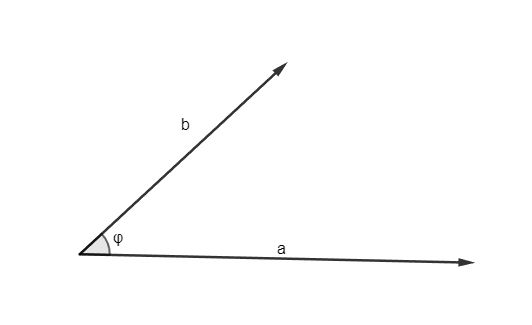
\includegraphics[height=7cm]{Images/Chapter_1/1-4-1.png}
\end{center}

\(\vec a \nparallel \vec b\). Если \(\vec a \parallel \vec b\), то \(\vec a \times \vec b = \vec 0\)

Свойства: (\(\forall \vec a, \vec b \in V_3\))
\begin{enumerate}
    \item Антисимметричность: \(\vec a \times \vec b = -\vec b \times \vec a\)

          Очевидно
    \item Аддитивность по 1-му аргументу: \(\forall \vec a_1, \vec a_2 \in V_3:
          (\vec a_1 + \vec a_2) \times \vec b = \vec a_1 \times \vec b + \vec a_2 \times \vec b\)

          Доказательство см. в 1.6
    \item Однородность по 1-му аргументу: \(\forall \lambda \in \mathbb{R}: (\lambda \vec a)\times \vec b = \lambda(\vec a \times \vec b)\)

          Очевидно
    \item \(|\vec a \times \vec b| = S(\text{параллелограмм, построенный на } \vec a, \vec b)\)

          Очевидно
\end{enumerate}

\(\begin{rcases*}
    2. \\
    3.
\end{rcases*} \Rightarrow\) Векторное произведение линейно по 1-му аргументу.

Координатное представление:

\(\vec a = (a_1, a_2, a_3) = a_1\vec i + a_2\vec j + a_3\vec k\)

\(\vec b = (b_1, b_2, b_3) = b_1\vec i + b_2\vec j + b_3\vec k\)

\(\vec c = (c_1, c_2, c_3) = c_1\vec i + c_2\vec j + c_3\vec k\)

\(\vec a \times \vec b = (a_1\vec i + a_2\vec j + a_3\vec k) \times (b_1\vec i + b_2\vec j + b_3\vec k) = \text{(пользуясь 1. -- 4.)} = \\
= a_1 b_1 (\vec i \times \vec i) + a_1 b_2 (\vec i \times \vec j) + a_1 b_3 (\vec i \times \vec k) + \\
+ a_2 b_1 (\vec j \times \vec i) + a_2 b_2 (\vec j \times \vec j) + a_2 b_3 (\vec j \times \vec k) + \\
+ a_3 b_1 (\vec k \times \vec i) + a_3 b_2 (\vec k \times \vec j) + a_3 b_3 (\vec k \times \vec k) = \\
= (\vec i \times \vec i = \vec j \times \vec j = \vec k \times \vec k = \vec 0; \\
\vec i \times \vec j = -(\vec j \times \vec i) = \vec k; \\
\vec k \times \vec i = -(\vec i \times \vec k) = \vec j; \\
\vec j \times \vec k = -(\vec k \times \vec j) = \vec i) = \\
= (a_2 b_3 - a_3 b_2)\vec i + (a_3 b_1 - a_1 b_3)\vec j + (a_1 b_2 - a_2 b_1)\vec k =
\begin{vmatrix}
    \vec i & \vec j & \vec k \\
    a_1    & a_2    & a_3    \\
    b_1    & b_2    & b_3
\end{vmatrix} = \vec i A_{11} + \vec j A_{12} + \vec k A_{13} = \\
= \left(
\begin{vmatrix}
        a_2 & a_3 \\
        b_2 & b_3
    \end{vmatrix}
, -
\begin{vmatrix}
        a_1 & a_3 \\
        b_1 & b_3
    \end{vmatrix}
,
\begin{vmatrix}
        a_1 & a_2 \\
        b_1 & b_2
    \end{vmatrix}
\right) =
(a_2 b_3 - a_3 b_2, a_3 b_1 - a_1 b_3, a_1 b_2 - a_2 b_1)\)


\subsection{Смешанное произведение векторов}
\(V_3 \times V_3 \times V_3 \rightarrow \mathbb{R}\)

Обозначения нет, вектора ставятся друг к другу без дополнительных знаков.

\(\vec a, \vec b, \vec c \in V_3 \rightarrow \vec a \vec b \vec c \in \mathbb{R}\)

\(\vec a \vec b \vec c \defeq (\vec a \times \vec b) \cdot \vec c\)

Свойства:
\begin{enumerate}
    \item \(|\vec a \vec b \vec c| = V(\text{параллелепипед, построенный на } \vec a, \vec b, \vec c)\),
          причём \(\vec a \vec b \vec c > 0 \Leftrightarrow \vec a, \vec b, \vec c\) --- правая тройка,
          \(\vec a \vec b \vec c < 0 \Leftrightarrow \vec a, \vec b, \vec c\) --- левая тройка.

          \begin{center}
              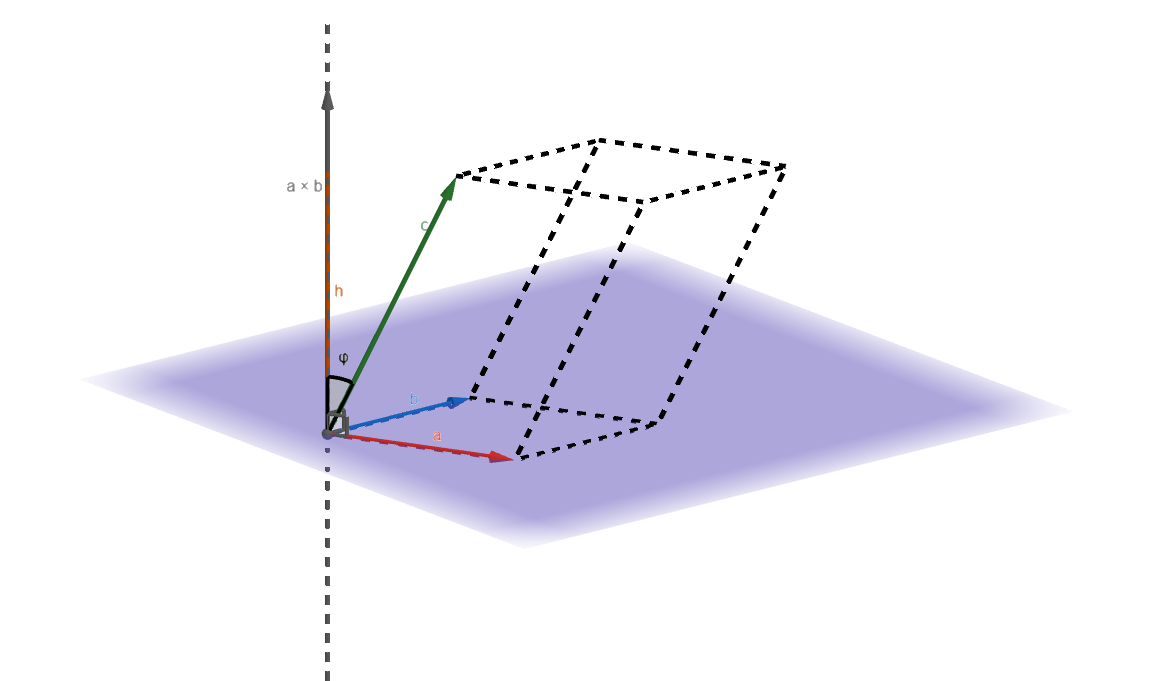
\includegraphics[height=7cm]{Images/Chapter_1/1-6-1.png}
          \end{center}

          \(\vec a \vec b \vec c = (\vec a \times \vec b) \cdot \vec c\),
          пусть \(\vec a \neq \vec 0\), \(\vec b \neq \vec 0\), \(\vec c \neq \vec 0\) (Если какой-либо вектор --- нулевой, то и произведение, и объём --- тоже нулевые)

          Пусть \(\vec a \nparallel \vec b\) (Иначе и произведение, и объём равны нулю)

          Построим \(\vec a \times \vec b\)
          \begin{itemize}
              \item \(\vec a, \vec b, \vec c\) --- правая тройка \(\Leftrightarrow \varphi = \angle(\vec a \times \vec b, \vec c) < 90^{\circ} \Leftrightarrow \cos\varphi > 0 \Leftrightarrow \vec a \vec b \vec c > 0\)
              \item \(\vec a, \vec b, \vec c\) --- левая тройка \(\Leftrightarrow \varphi = \angle(\vec a \times \vec b, \vec c) > 90^{\circ} \Leftrightarrow \cos\varphi < 0 \Leftrightarrow \vec a \vec b \vec c < 0\)
          \end{itemize}

          \(V := V(\text{параллелепипед, построенный на } \vec a, \vec b, \vec c) = \\
          = S(\text{параллелограмм, построенный на } \vec a, \vec b) \cdot h\), где \(h\) - высота параллелограмма.

          \(h = |\proj_{\vec a \times \vec b}\vec c| = ||\vec c| \cos \varphi|\)

          \(S(\text{параллелограмм, построенный на } \vec a, \vec b) = |\vec a \times \vec b|\)

          \(V = |\vec a \times \vec b| \cdot ||\vec c| \cos \varphi| = |(\vec a \times \vec b) \cdot \vec c| = |\vec a \vec b \vec c|\) \(Q.E.D.\)
    \item \(\vec a \vec b \vec c = \vec b \vec c \vec a = \vec c \vec a \vec b = -\vec c \vec b \vec a = -\vec b \vec a \vec c = -\vec a \vec c \vec b\)

          \(\vec a, \vec b, \vec c\) --- правая тройка \(\Leftrightarrow \vec a \vec b \vec c = V(\text{параллелепипед, построенный на } \vec a, \vec b, \vec c)\),
          а объём не зависит от того, какой вектор выбрать первым, значит:

          \(V = \vec a \vec b \vec c = \vec b \vec c \vec a = \vec c \vec a \vec b\)

          То же самое, если \(\vec a, \vec b, \vec c\) --- левая тройка, но со знаком минус.

    \item Аддитивность по первому (с 2., по любому) аргументу:
          \((\vec a_1 + \vec a_2)\vec b \vec c = \vec a_1 \vec b \vec c + \vec a_2 \vec b \vec c\)

          \((\vec a_1 + \vec a_2)\vec b \vec c = (\text{по 2.}) = \vec b \vec c (\vec a_1 + \vec a_2) =
          (\vec b \times \vec c) \cdot (\vec a_1 + \vec a_2) =
          (\vec b \times \vec c) \cdot \vec a_1 + (\vec b \times \vec c) \cdot \vec a_2 =
          \vec b \vec c \vec a_2 + \vec b \vec c \vec a_1 = (\text{по 2.}) =
          \vec a_1 \vec b \vec c + \vec a_2 \vec b \vec c\) \(Q.E.D.\)
    \item Однородность по первому (с 2., по любому) аргументу:
          \((\lambda\vec a)\vec b \vec c = \lambda(\vec a \vec b \vec c)\)

          \((\lambda\vec a)\vec b \vec c = (\text{по 2.}) = \vec b \vec c (\lambda\vec a) =
          (\vec b \times \vec c) \cdot (\lambda\vec a) =
          \lambda((\vec b \times \vec c) \cdot \vec a) =
          \lambda(\vec b \vec c \vec a) = (\text{по 2.}) =
          \lambda(\vec a \vec b \vec c)\) \(Q.E.D.\)
\end{enumerate}

Координатное представление:

\(\vec a \vec b \vec c = (\vec a \times \vec b) \cdot \vec c =
\begin{vmatrix}
    \vec i & \vec j & \vec k \\
    a_1    & a_2    & a_3    \\
    b_1    & b_2    & b_3
\end{vmatrix} \cdot \vec c =
\begin{vmatrix}
    c_1 & c_2 & c_3 \\
    a_1 & a_2 & a_3 \\
    b_1 & b_2 & b_3
\end{vmatrix} =
\begin{vmatrix}
    a_1 & a_2 & a_3 \\
    b_1 & b_2 & b_3 \\
    c_1 & c_2 & c_3
\end{vmatrix}\)

Доказательство аддитивности векторного произведения:

\(\forall \vec a_1, \vec a_2, \vec b \in V_3\)

\((\vec a_1 + \vec a_2)\vec b \vec c = ((\vec a_1 + \vec a_2) \times \vec b) \cdot \vec c = \vec a_1 \vec b \vec c + \vec a_2 \vec b \vec c\)

Пусть \(\vec c = \vec i\). Тогда: \((\vec a_1 + \vec a_2)\vec b \vec c = ((\vec a_1 + \vec a_2) \times \vec b) \cdot \vec i = ((\vec a_1 + \vec a_2) \times \vec b)_x\)

\(m = 1, 2:\; (\vec a_m \times \vec b) \cdot \vec c = (\vec a_m \times \vec b) \cdot \vec i = (\vec a_m \times \vec b)_x\)

\((\vec a_1 + \vec a_2)\vec b \vec c = \vec a_1 \vec b \vec c + \vec a_2 \vec b \vec c \Leftrightarrow ((\vec a_1 + \vec a_2) \times \vec b)_x = (\vec a_1 \times \vec b)_x + (\vec a_2 \times \vec b)_x\)

Повторим то же самое, но с \(\vec c = \vec j\) и \(\vec c = \vec k\).

\(\begin{rcases}
    ((\vec a_1 + \vec a_2) \times \vec b)_x = (\vec a_1 \times \vec b)_x + (\vec a_2 \times \vec b)_x \\
    ((\vec a_1 + \vec a_2) \times \vec b)_y = (\vec a_1 \times \vec b)_y + (\vec a_2 \times \vec b)_y \\
    ((\vec a_1 + \vec a_2) \times \vec b)_z = (\vec a_1 \times \vec b)_z + (\vec a_2 \times \vec b)_z
\end{rcases} \Leftrightarrow (\vec a_1 + \vec a_2) \times \vec b = (\vec a_1 \times \vec b) + (\vec a_2 \times \vec b)\) \(Q.E.D.\)

Двойное векторное произведение

\(\vec a \times (\vec b \times \vec c) = \vec b(\vec a \cdot \vec c) - \vec c(\vec a \cdot \vec b)\)
\begin{itemize}
    \item \(\vec b \nparallel \vec c\):
          \begin{center}
              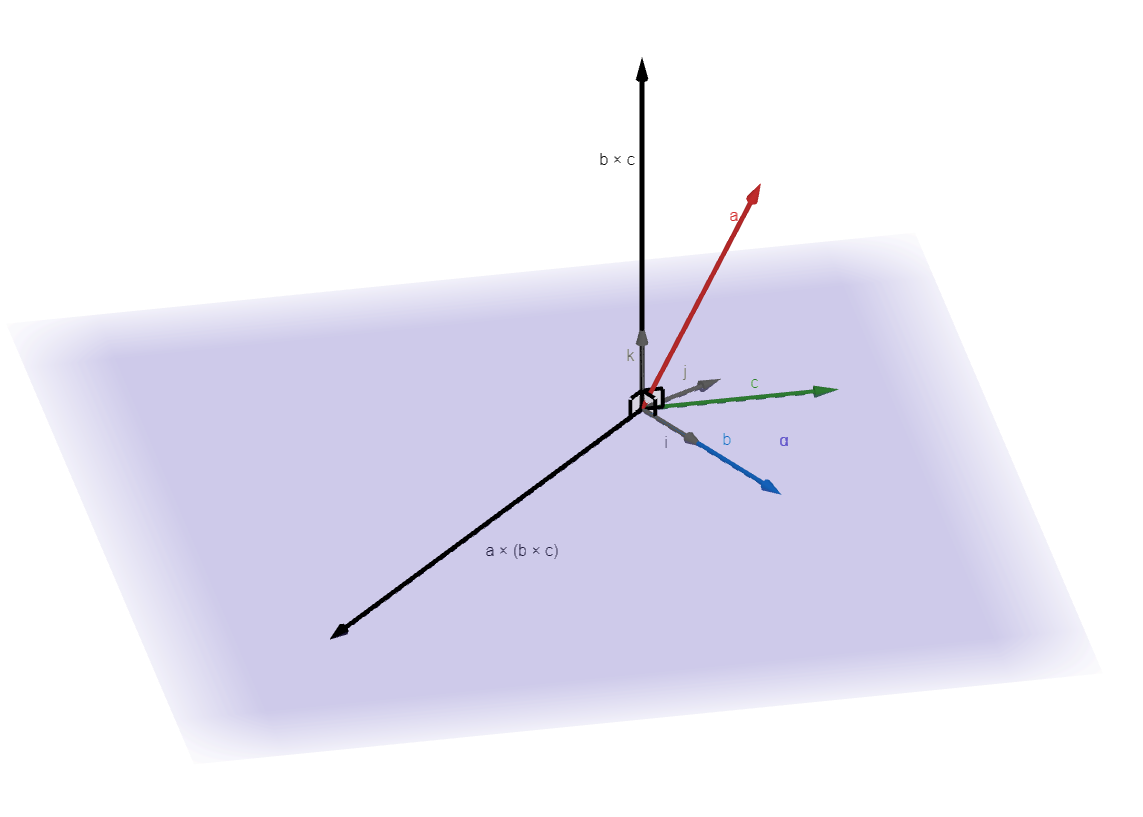
\includegraphics[height=7cm]{Images/Chapter_1/1-7-1.png}
          \end{center}
          Проведём плоскость \(\alpha(\vec b, \vec c) \Rightarrow \vec b \times \vec c \perp \alpha\)

          \(\vec a \times (\vec b \times \vec c) \perp \vec b \times \vec c \Rightarrow \vec a \times (\vec b \times \vec c) \in \alpha\)

          Введём ДСК, где \(\vec i = \frac{\vec b}{|\vec b|}\), \(\vec j \in \alpha\), \(\vec k \perp \alpha\). Тогда:

          \(\vec b = (b_1, 0, 0);\; \vec c = (c_1, c_2, 0);\; \vec a = (a_1, a_2, a_3)\)

          \(\vec b \times \vec c = (b_1, 0, 0) \times (c_1, c_2, 0) = (0, 0, b_1 c_2)\)

          \(\vec a \times (\vec b \times \vec c) = (a_1, a_2, a_3) \times (0, 0, b_1 c_2) = (a_2 b_1 c_2, -a_1 b_1 c_2, 0)\)

          \(\vec b(\vec a \cdot \vec c) - \vec c(\vec a \cdot \vec b) = \vec b a_1 c_1 + \vec b a_2 c_2 - \vec c a_1 b_1 =
          (b_1(a_1 c_1 + a_2 c_2) - c_1 a_1 b_1, -c_2 a_1 b_1, 0) =
          (a_2 b_1 c_2, -a_1 b_1 c_2, 0) = \vec a \times (\vec b \times \vec c)\) \(Q.E.D.\)
    \item \(\vec b \parallel \vec c\):

          \(\vec b \times \vec c = \vec 0\)

          \(\exists \lambda \in \mathbb{R}: \vec b = \lambda \vec c\)

          \(\begin{rcases}
              \vec b(\vec a \cdot \vec c) = \lambda c(\vec a \cdot \vec c) \\
              \vec c(\vec a \cdot \vec b) = \vec c(\vec a \cdot \lambda\vec c) = \lambda \vec c(\vec a \cdot \vec c)
          \end{rcases} \Rightarrow \vec b(\vec a \cdot \vec c) - \vec c(\vec a \cdot \vec b) = \vec 0 = \vec b \times \vec c\) \(Q.E.D.\)
\end{itemize}

\newpage 

\section{Прямая на плоскости, плоскость и прямая в пространстве}
\subsection{Линейное уравнение}

На плоскости (в пространстве) в ДСК \(Oxy\) (\(Oxyz\)) уравнение \(Ax + By + C = 0\), \(A^2 + B^2 \neq 0\) (\(Ax + By + Cz + D = 0\), \(A^2 + B^2 + C^2 \neq 0\)) --- алгебраическое уравнение первого порядка или линейное уравнение.

Любое линейное уравнение на плоскости (в пространстве) определяет прямую (плоскость), и наоборот, любая прямая (плоскость) на плоскости (в пространстве) может быть описана линейным уравнением.

Доказывать будем для прямой в плоскости. Доказательство для прямой в пространстве полностью аналогично.
\begin{enumerate}
    \item Уравнение \(\rightarrow\) прямая:
          \begin{center}
              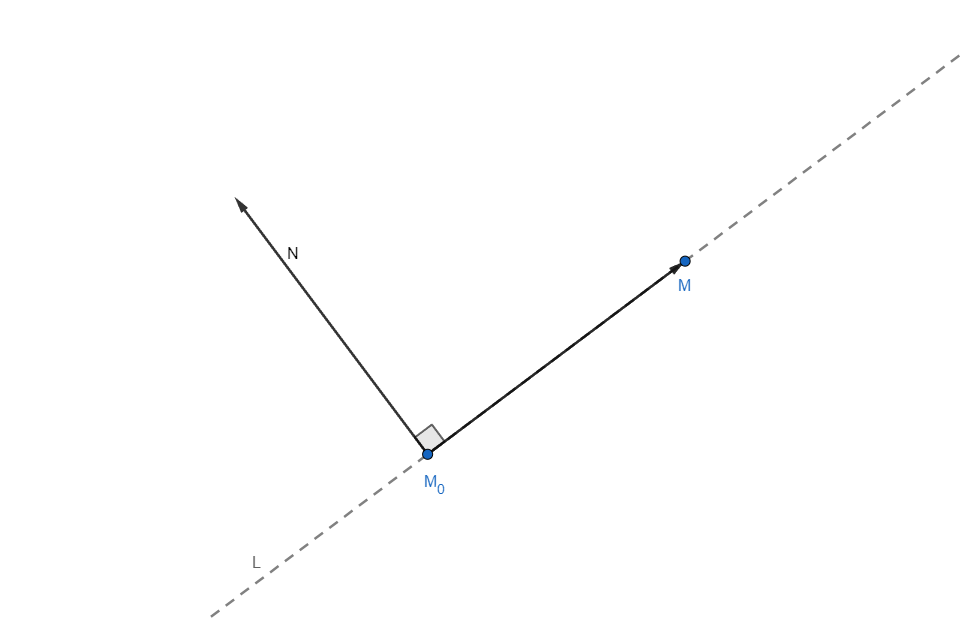
\includegraphics[height=7cm]{Images/Chapter_1/2-1-1.png}
          \end{center}
          \(Ax + By + C = 0\), \(A^2 + B^2 \neq 0\)
          Не умаляя общности, пусть \(B \neq 0\). Тогда \(M_0(x_0, y_0) = (0, \frac{-C}{B})\) - удовлетворяет уравнению.

          Пусть \(M(x, y) \neq M\) - тоже удовлетворяет уравнению. Тогда \(A(x - x_0) + B(y - y_0) = 0\).

          \(\overrightarrow{M_0 M} = (x - x_0, y - y_0)\)

          \(\vec N := (A, B) \neq 0\)

          \(M_0(x_0, y_0) = (0, \frac{-C}{B}) \Leftrightarrow \overrightarrow{M_0 M} \cdot \vec N = 0 \Leftrightarrow \vec N \perp \overrightarrow{M_0 M} \Rightarrow \\
          \Rightarrow \forall M(x, y) \text{, удовлетворяющих } A(x - x_0) + B(y - y_0) = 0: M \in L \perp \vec N, M_0 \in L\)

          И наоборот, если \(M \in L\), то \(\overrightarrow{M_0 M} \perp \vec N \Rightarrow M \text{ удовлетворяет } A(x - x_0) + B(y - y_0) = 0\)

          \(Ax + By + C = 0\) Определяет прямую \(L\) и никакую другую, т.к. Если \(M \notin L\), то \(\overrightarrow{M_0 M} \not\perp \vec N \Rightarrow M \text{ не удовлетворяет } A(x - x_0) + B(y - y_0) = 0\) \(Q.E.D.\)
    \item Прямая \(\rightarrow\) уравнение:
          \begin{center}
              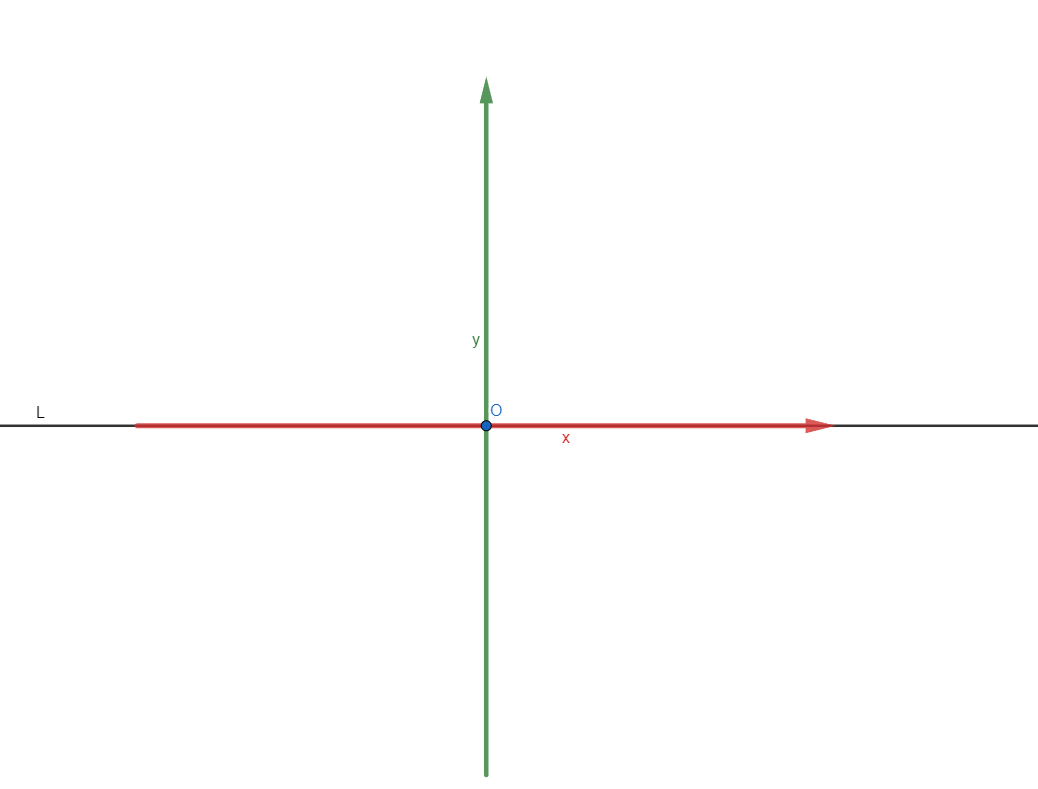
\includegraphics[height=7cm]{Images/Chapter_1/2-1-2.png}
          \end{center}
          Пусть \(L\) --- прямая на плоскости.

          Введём ДСК так, чтобы \(L\) совпадала с \(Ox\). Тогда очевидно, что линейное уравнение \(y = 0\) содержит все точки \(L\).

          Если есть ДСК, в которой \(L\) задаётся линейным уравнением, то в любой другой ДСК \(L\) будет задаваться линейным уравнением.
          Любые две ДСК связаны поворотом и сдвигом, значит нужно доказать, что при повороте и сдвиге линейное уравнение остаётся линейным уравнением.

          \begin{itemize}
              \item Сдвиг:
                    \begin{center}
                        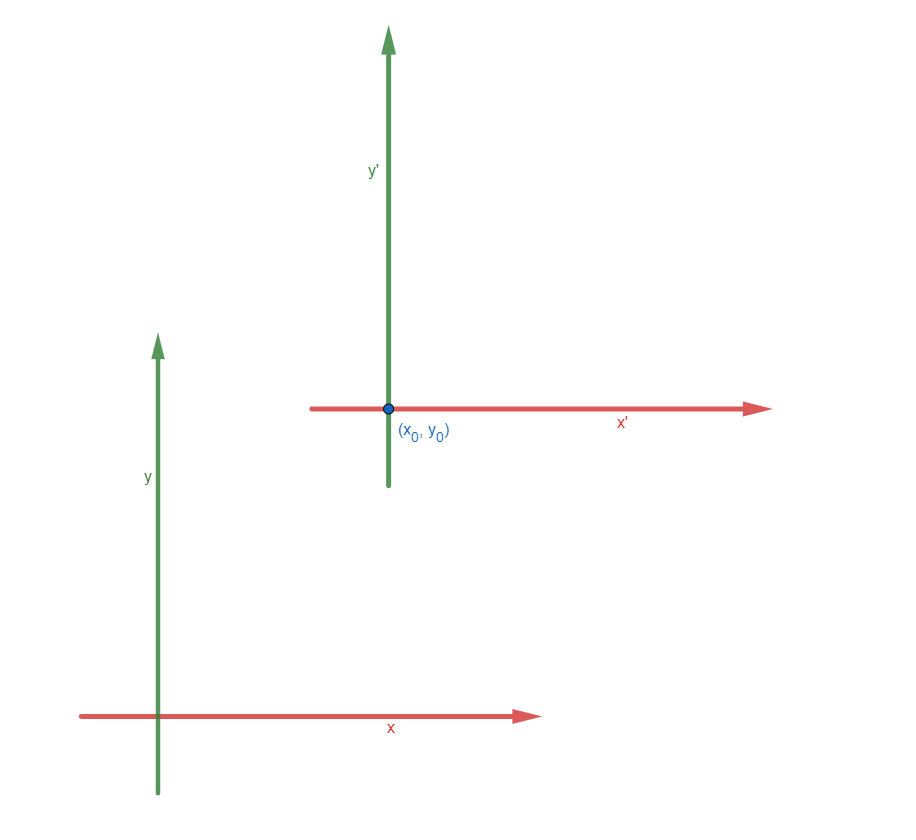
\includegraphics[height=7cm]{Images/Chapter_1/2-1-3.png}
                    \end{center}
                    \(x = x' + x_0\)

                    \(y = y' + y_0\)

                    \(A(x' + x_0) + B(y' + y_0) + C = 0 \Rightarrow Ax' + By' + (Ax_0 + By_0 + C) = 0\)

                    \(C' := (Ax_0 + By_0 + C)\)

                    \(Ax + By + C' = 0\) - тоже линейное уравнение.
              \item Поворот:
                    \begin{center}
                        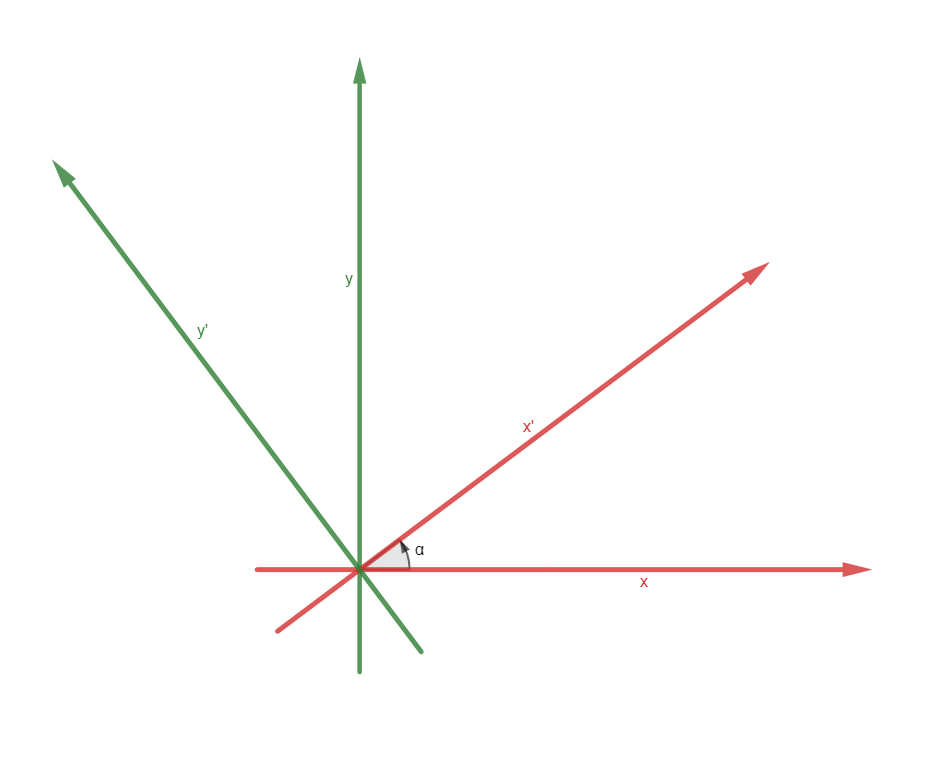
\includegraphics[height=7cm]{Images/Chapter_1/2-1-4.png}
                    \end{center}
                    \(x = x'\cos\alpha - y'\sin\alpha\)

                    \(y = x'\sin\alpha + y'\cos\alpha\)

                    \(A(x'\cos\alpha - y'\sin\alpha) + B(x'\sin\alpha + y'\cos\alpha) + C = 0 \Rightarrow (A\cos\alpha + B\sin\alpha)x' + (B\cos\alpha - A\sin\alpha)y' + C = 0\)

                    \(A' := A\cos\alpha + B\sin\alpha\)

                    \(B' := B\cos\alpha - A\sin\alpha\)

                    \(A'^2 + B'^2 = A^2 + B^2 \neq 0\), значит \(A'x + B'y + C = 0\) - тоже линейное уравнение.
          \end{itemize}
          Значит если прямая задаётся линейным уравнением в ДСК, то в любой другой ДСК эта прямая будет задаваться линейным уравнением \(\quad Q.E.D.\)
\end{enumerate}

\(Ax + By + C = 0\), \(A^2 + B^2 \neq 0\) --- Общее уравнение прямой на плоскости, \(\vec N = (A, B)\) --- Вектор нормали.

\(Ax + By + Cz + D = 0\), \(A^2 + B^2 + C^2\neq 0\) --- Общее уравнение плоскости в пространстве, \(\vec N = (A, B, C)\) --- Вектор нормали.

\subsection{Способы задания}
\begin{center}
    \begin{longtable}[t]{|p{5.5cm}|p{5.5cm}|p{5.5cm}|}
        \hline
        Прямая в плоскости
         &
        Плоскость в пространстве
         &
        Прямая в пространстве
        \\
        \hline
        Общее уравнение:
        \begin{center}
            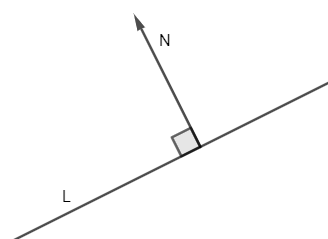
\includegraphics[width=5.5cm]{Images/Chapter_1/2-2-1.png}
        \end{center}
        \fbox{\(Ax + By + C = 0\)}

        \(A^2 + B^2 \neq 0\)

        \(\vec N = (A, B)\) --- нормаль. \(\vec N \perp L\).

        \(C = 0 \Rightarrow L \cap (0, 0)\)
         &
        Общее уравнение:
        \begin{center}
            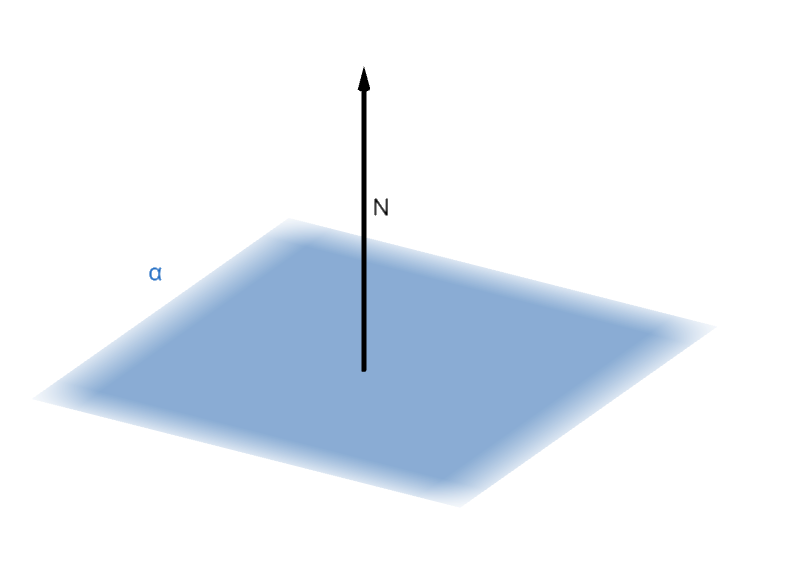
\includegraphics[width=5.5cm]{Images/Chapter_1/2-2-10.png}
        \end{center}
        \fbox{\(Ax + By + Cz + D = 0\)}

        \(A^2 + B^2 + C^2 \neq 0\)

        \(\vec N = (A, B, C)\) --- нормаль. \(\vec N \perp \alpha\).

        \(C = 0 \Rightarrow \alpha \cap (0, 0, 0)\)
         &
        Пересечение плоскостей:
        \begin{center}
            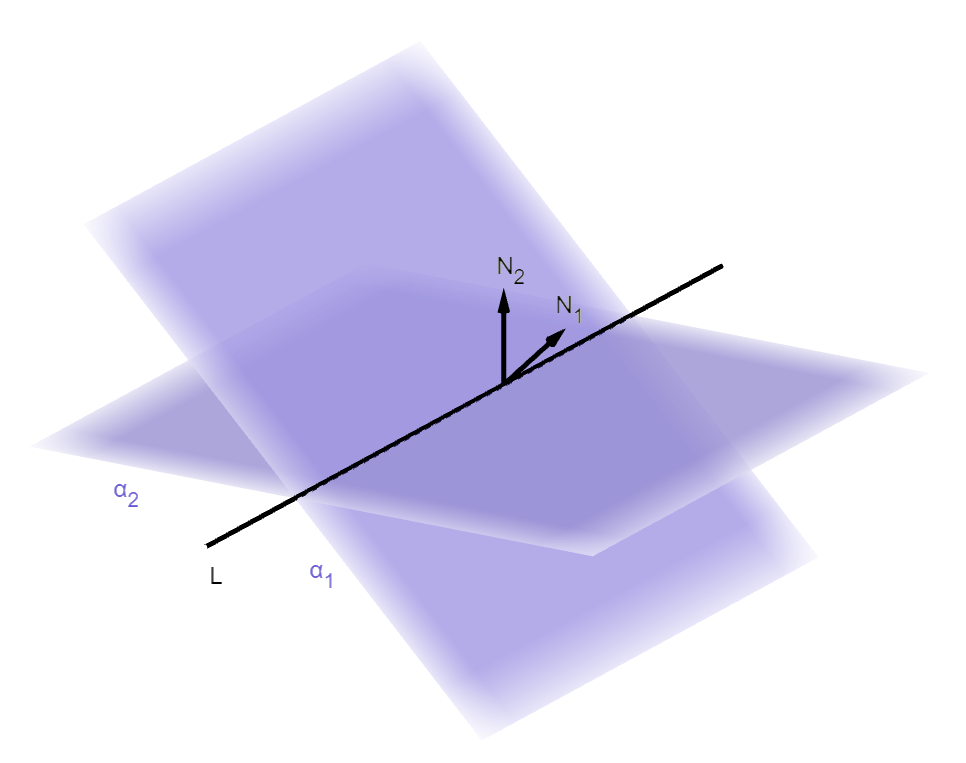
\includegraphics[width=5.5cm]{Images/Chapter_1/2-2-18.png}
        \end{center}
        \(L = \alpha_1 \cap \alpha_2\)

        \scriptsize\fbox{\(L:
            \begin{cases}
                A_1 x + B_1 y + C_1 z + D_1 = 0 \\
                A_2 x + B_2 y + C_2 z + D_2 = 0
            \end{cases}\)}\normalsize

        \(A_i^2 + B_i^2 + C_i^2 \neq 0\)

        \(\vec N_1 \nparallel \vec N_2\)
        \\
        \hline
        Уравнение в отрезках:
        \begin{center}
            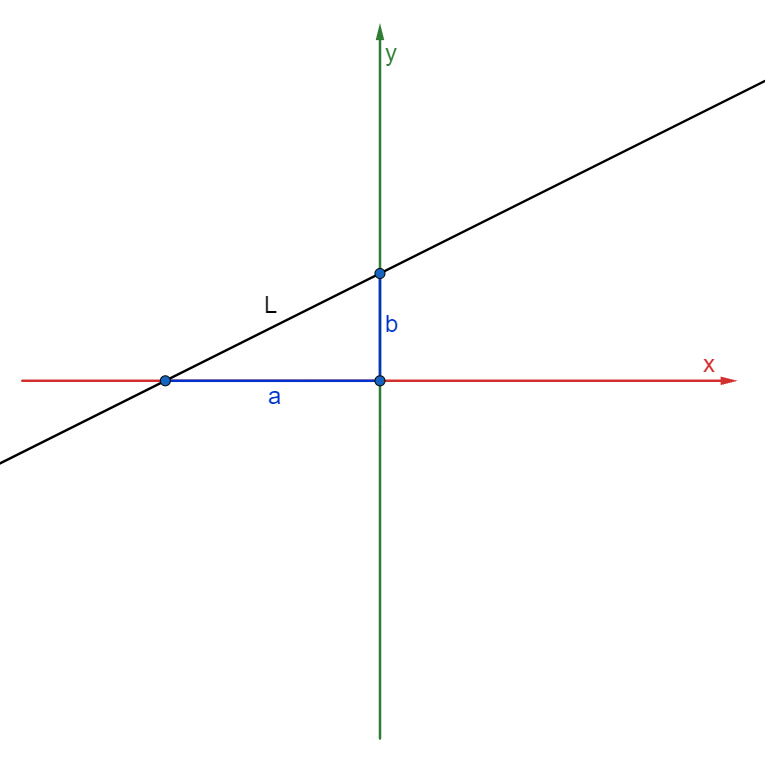
\includegraphics[width=5.5cm]{Images/Chapter_1/2-2-2.png}
        \end{center}
        \((0, 0) \notin L\)

        \fbox{\(\dfrac{x}{a} + \dfrac{y}{b} = 1\)}

        \(a^2 + b^2 \neq 0\)
         &
        Уравнение в отрезках:
        \begin{center}
            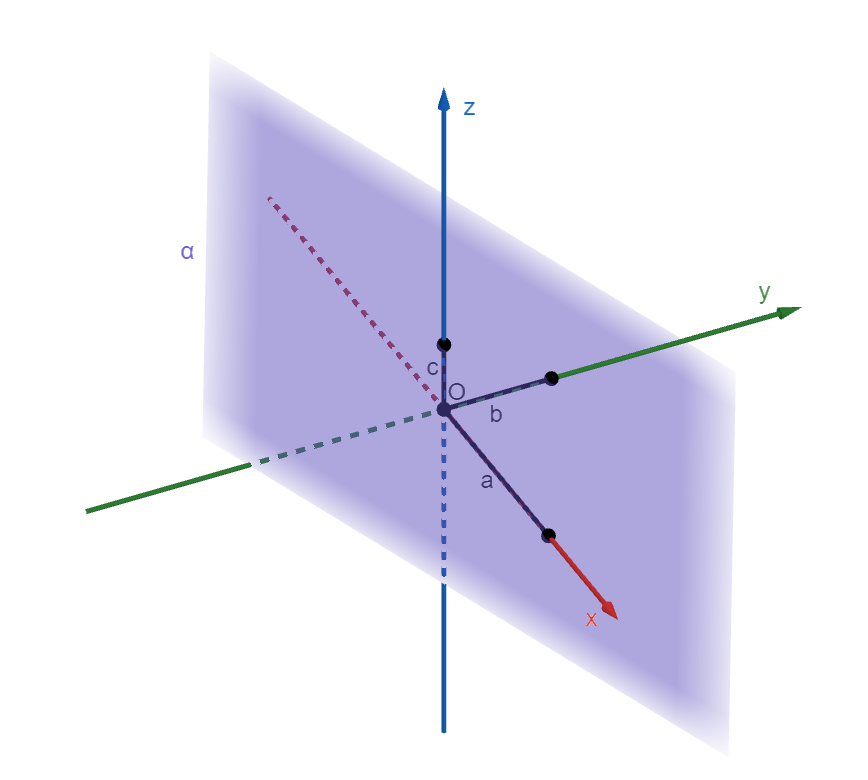
\includegraphics[width=5.5cm]{Images/Chapter_1/2-2-11.png}
        \end{center}
        \((0, 0, 0) \notin \alpha\)

        \fbox{\(\dfrac{x}{a} + \dfrac{y}{b} + \dfrac{z}{c} = 1\)}

        \(a^2 + b^2 + c^2 \neq 0\)
         &
        Пересечение плоскостей \(\rightarrow\) каноническое уравнение:
        \begin{center}
            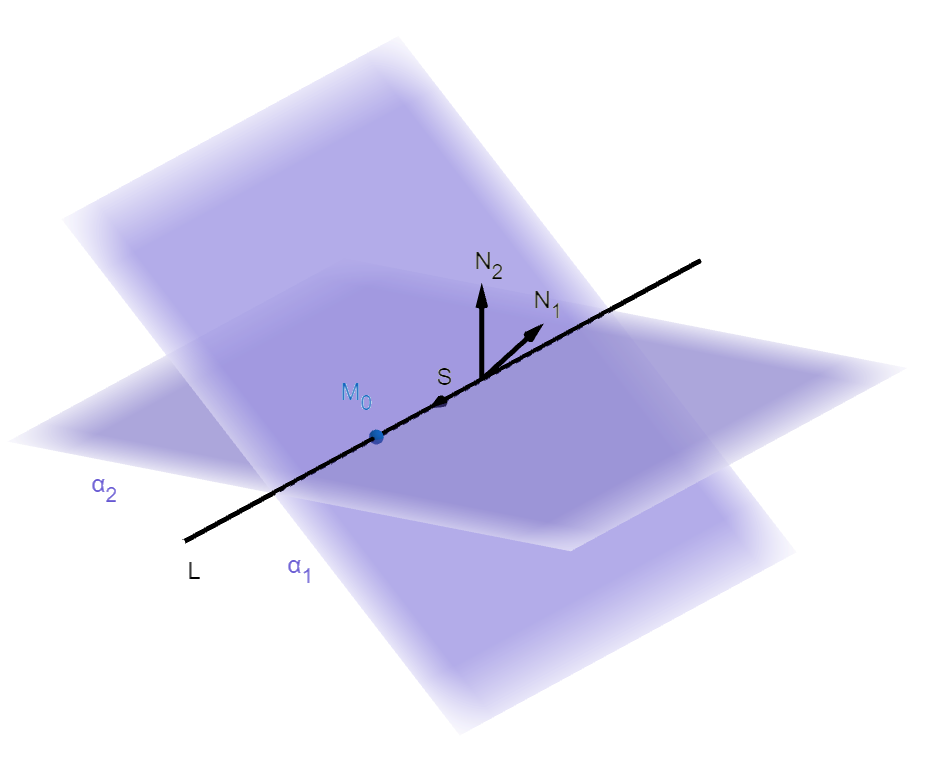
\includegraphics[width=5.5cm]{Images/Chapter_1/2-2-19.png}
        \end{center}
        \(\vec S \perp \vec N_1, \vec S \perp \vec N_2\)

        \(\vec S = \vec N_1 \times \vec N_2\)

        Пусть \(M_0 = (x_0, y_0, 0) = L \cap Oz\)

        Тогда решим систему:

        \small\fbox{\(L:
            \begin{cases}
                A_1 x_0 + B_1 y_0 + D_1 = 0 \\
                A_2 x_0 + B_2 y_0 + D_2 = 0
            \end{cases}\)}\normalsize

        Если не получилось, то \(M_0 = (x_0, 0, z_0) = L \cap Oy\)

        Cнова не получилось: \(M_0 = (0, y_0, z_0) = L \cap Ox\)
        \\
        \hline
        Уравнение через нормаль и точку:
        \begin{center}
            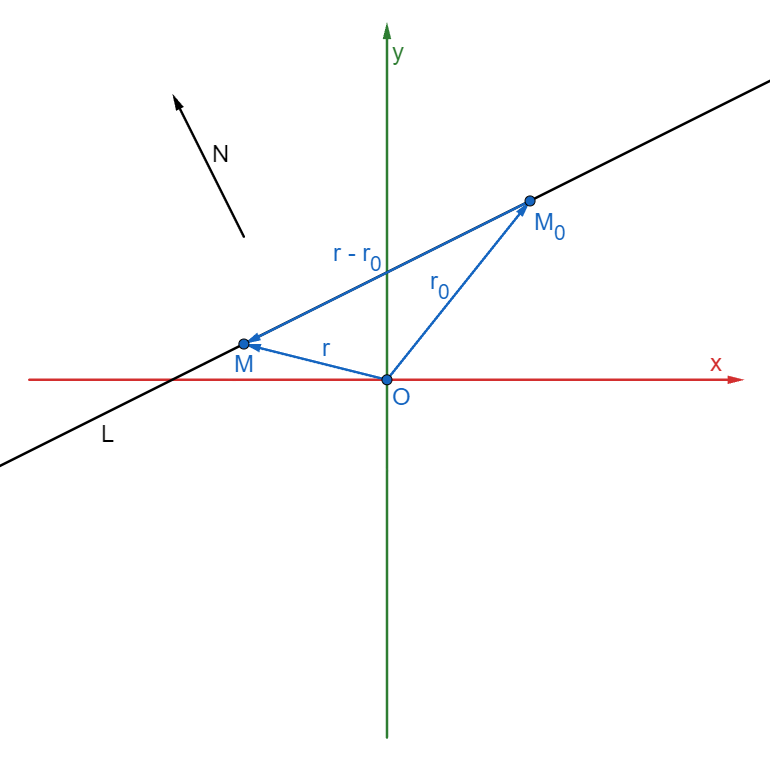
\includegraphics[width=5.5cm]{Images/Chapter_1/2-2-3.png}
        \end{center}
        \(M_0(x_0, y_0) \in L\)

        \(\vec N(A, B) \perp L\)

        \(M(x, y) \in L\)

        \(\vec r_0 = \overrightarrow{OM_0} = (x_0, y_0)\)

        \(\vec r = \overrightarrow{OM} = (x, y)\)

        \(\overrightarrow{M_0M} = \vec r - \vec r_0 \perp \vec N \Leftrightarrow\)

        \(\Leftrightarrow\) \fbox{\((\vec r - \vec r_0) \cdot \vec N = 0\)} \(\Leftrightarrow\)

        \small\(\Leftrightarrow\)\fbox{\(A(x - x_0) + B(y - y_0) = 0\)}\normalsize

        \(\)
         &
        Уравнение через нормаль и точку:
        \begin{center}
            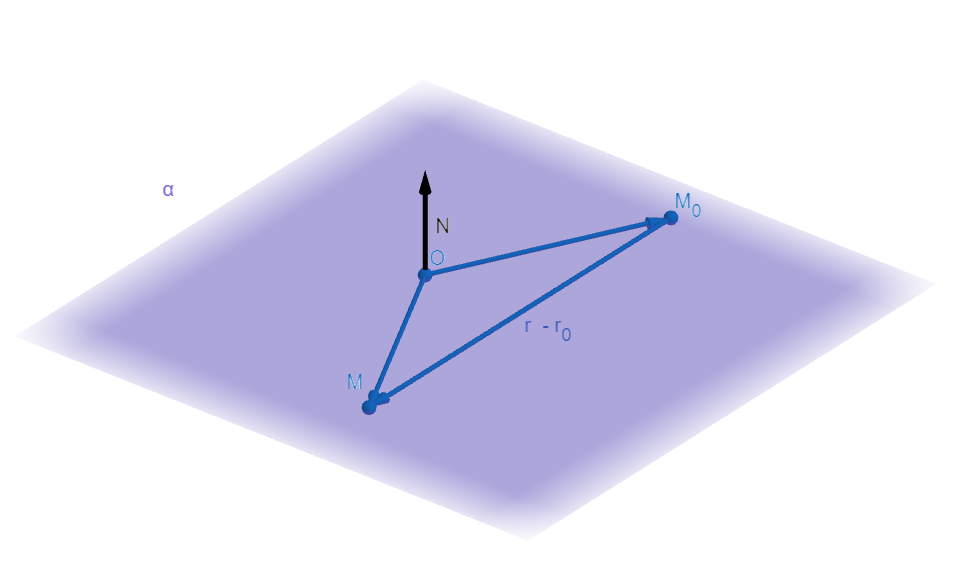
\includegraphics[width=5.5cm]{Images/Chapter_1/2-2-12.png}
        \end{center}
        \(M_0(x_0, y_0, z_0) \in \alpha\)

        \(\vec N(A, B, C) \perp \alpha\)

        \(M(x, y, z) \in \alpha\)

        \(\vec r_0 = \overrightarrow{OM_0} = (x_0, y_0, z_0)\)

        \(\vec r = \overrightarrow{OM} = (x, y, z)\)

        \(\overrightarrow{M_0M} = \vec r - \vec r_0 \perp \vec N \Leftrightarrow\)

        \(\Leftrightarrow\) \fbox{\((\vec r - \vec r_0) \cdot \vec N = 0\)}\(\Leftrightarrow\)

        \scriptsize\(\Leftrightarrow\)\fbox{\(A(x - x_0) + B(y - y_0) + C(z - z_0) = 0\)}\normalsize

        \(\)
         &
        Каноническое уравнение \(\rightarrow\) пересечение плоскостей:

        \scriptsize\(L:
        \begin{cases}
            l(x - x_0) + m(y - y_0) = 0 \\
            l(x - x_0) + n(z - z_0) = 0
        \end{cases}\)\normalsize

        Где \((l, m, n) = \vec S\) - направляющий вектор прямой \(L\),

        \((x_0, y_0, z_0) = M_0 \in L\)
        \\
        \hline
        Каноническое / параметрическое уравнение:
        \begin{center}
            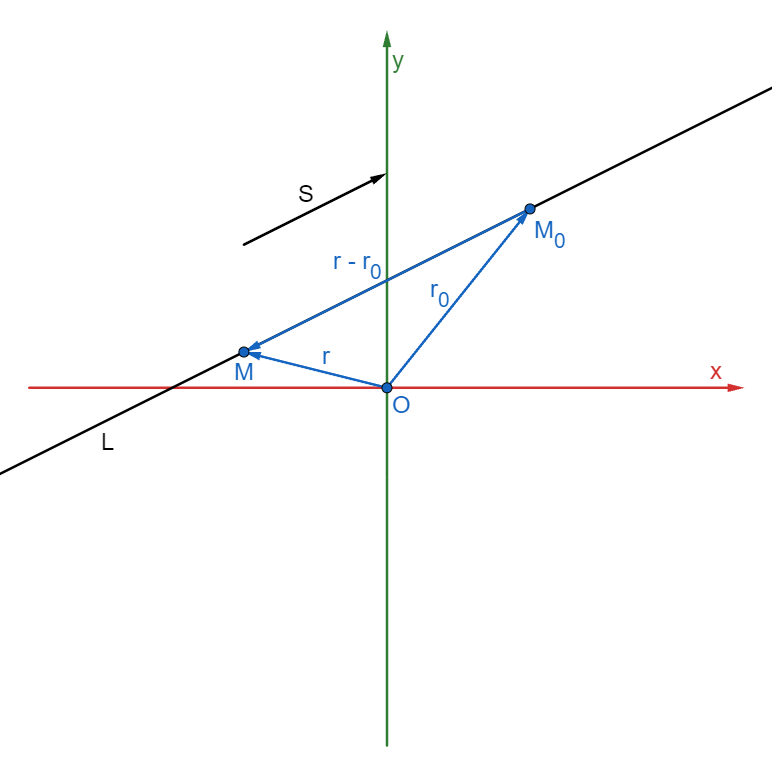
\includegraphics[width=5.5cm]{Images/Chapter_1/2-2-4.png}
        \end{center}
        \(M_0(x_0, y_0) \in L\)

        \(\vec S(l, m) \parallel L\)

        \(M(x, y) \in L\)

        \(\vec r_0 = \overrightarrow{OM_0} = (x_0, y_0)\)

        \(\vec r = \overrightarrow{OM} = (x, y)\)

        \(\overrightarrow{M_0M} = \vec r - \vec r_0 \parallel \vec S \Leftrightarrow\)

        \(\Leftrightarrow \exists t \in \mathbb{R}: \vec r - \vec r_0 = t \vec S \Leftrightarrow\)

        \(\Leftrightarrow\)\fbox{\(\dfrac{x - x_0}{l} = \dfrac{y - y_0}{m} = t\)}

        \fbox{\(\vec r = \vec r_0 + t \vec S\)}

        \fbox{
            \(
            \begin{cases}
                x = x_0 + tl \\
                y = y_0 + tm
            \end{cases}
            \)
        }

        \(\)
         &
        Условие принадлежности четырёх точек плоскости:
        \begin{center}
            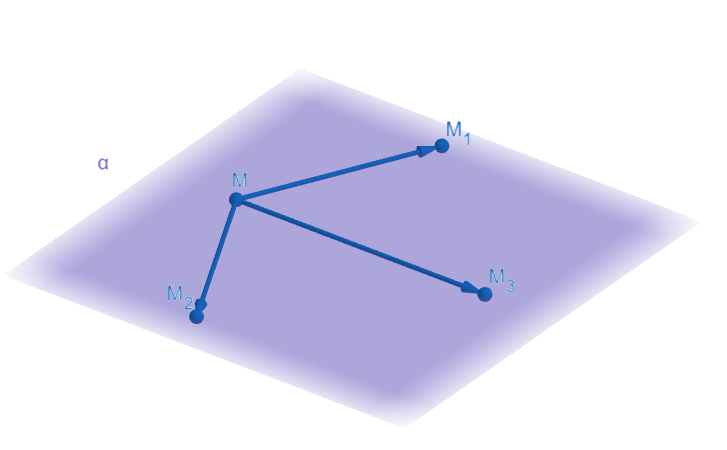
\includegraphics[width=5.5cm]{Images/Chapter_1/2-2-13.png}
        \end{center}
        \(M, M_1, M_2, M_3 \in \alpha\):

        \fbox{\(\overrightarrow{MM_1}\overrightarrow{MM_2}\overrightarrow{MM_3} = 0\)}
         &
        Каноническое / параметрическое уравнение:
        \begin{center}
            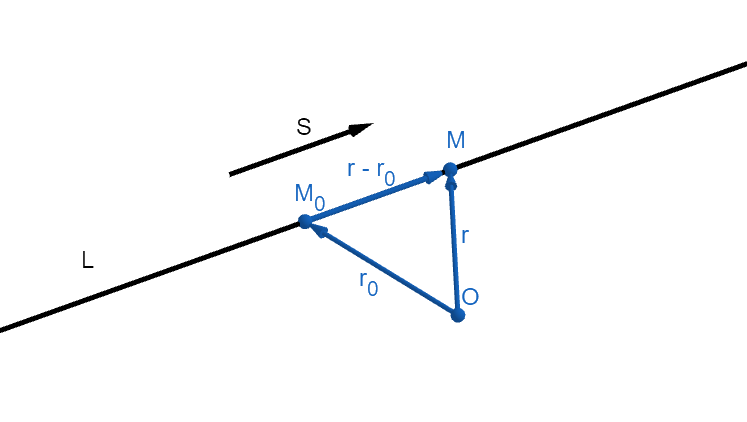
\includegraphics[width=5.5cm]{Images/Chapter_1/2-2-20.png}
        \end{center}
        \(M_0(x_0, y_0, z_0) \in L\)

        \(\vec S(l, m, n) \parallel L\)

        \(M(x, y, z) \in L\)

        \(\vec r_0 = \overrightarrow{OM_0} = (x_0, y_0, z_0)\)

        \(\vec r = \overrightarrow{OM} = (x, y, z)\)

        \(\overrightarrow{M_0M} = \vec r - \vec r_0 \parallel \vec S \Leftrightarrow\)

        \scriptsize\(\Leftrightarrow\)\fbox{\(\dfrac{x - x_0}{l} = \dfrac{y - y_0}{m} = \dfrac{z - z_0}{n} = t\)}\normalsize

        \fbox{\(\vec r = \vec r_0 + t \vec S\)}

        \fbox{
            \(
            \begin{cases}
                x = x_0 + tl \\
                y = y_0 + tm \\
                z = z_0 + tn
            \end{cases}
            \)
        }

        \(\)
        \\
        \hline
        Нормальное уравнение:
        \begin{center}
            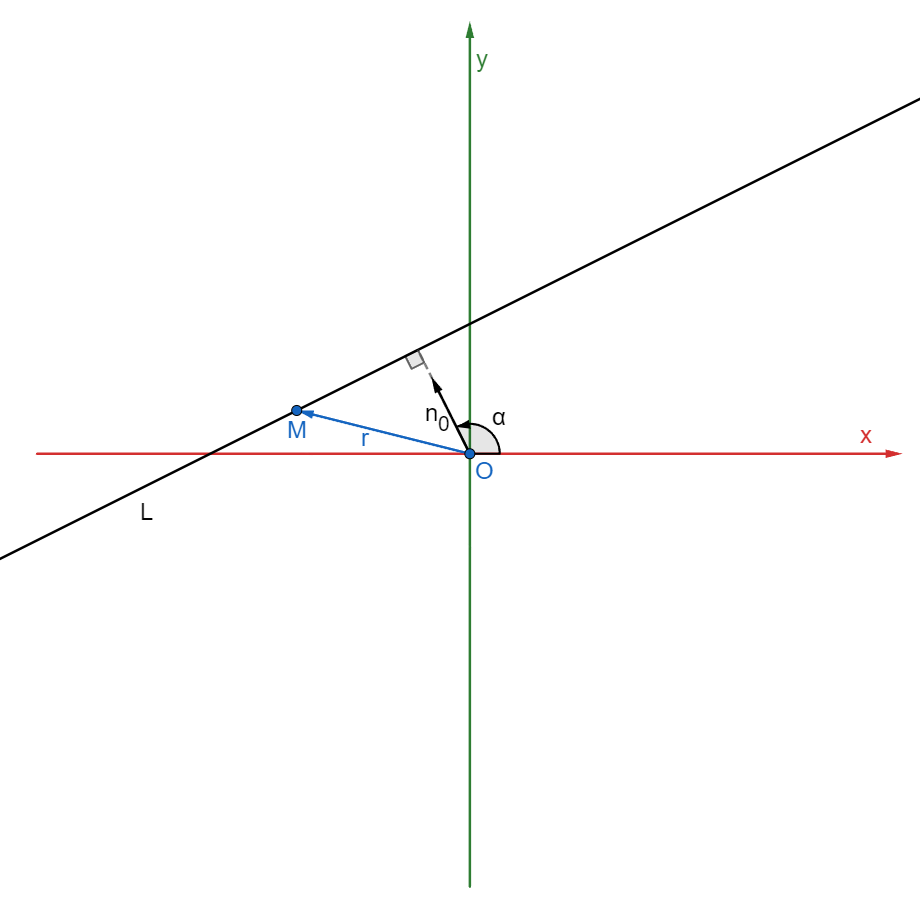
\includegraphics[width=5.5cm]{Images/Chapter_1/2-2-5.png}
        \end{center}
        \(O(0, 0) \notin L\)

        \(P = |O, L| > 0\)

        \(\vec n_0 \perp L\), \(|\vec n_0| = 1\)

        \(\vec n_0\) направлен в сторону \(L\) если его приложить к \(O\)

        \(\vec n_0 = (\cos \alpha, \sin \alpha)\)

        \(M(x, y) \in L\)

        \(P = \proj_{\vec n_0} \vec r \Leftrightarrow\)

        \(\Leftrightarrow\) \fbox{\(\vec r \cdot \vec n_0 - P = 0\)}

        \fbox{\(x \cos \alpha + y \sin \alpha - P = 0\)}

        \(L: Ax + By + C = 0\), \(A^2 + B^2 \neq 0\)

        \(\vec N = (A, B) \perp L \Rightarrow\)

        \(\Rightarrow \vec n_0 = \dfrac{\pm \vec N}{|\vec N|} = \)

        \small\(= \pm \left(\dfrac{A}{\sqrt{A^2 + B^2}}, \dfrac{B}{\sqrt{A^2 + B^2}}\right)\)\normalsize

        \(C > 0: ``+"\)

        \(C < 0: ``-"\)

        \(\cos \alpha = \dfrac{\pm A}{\sqrt{A^2 + B^2}}\)

        \(\sin \alpha = \dfrac{\pm B}{\sqrt{A^2 + B^2}}\)

        \(P = \dfrac{\pm C}{\sqrt{A^2 + B^2}}\)
         &
        Нормальное уравнение:
        \begin{center}
            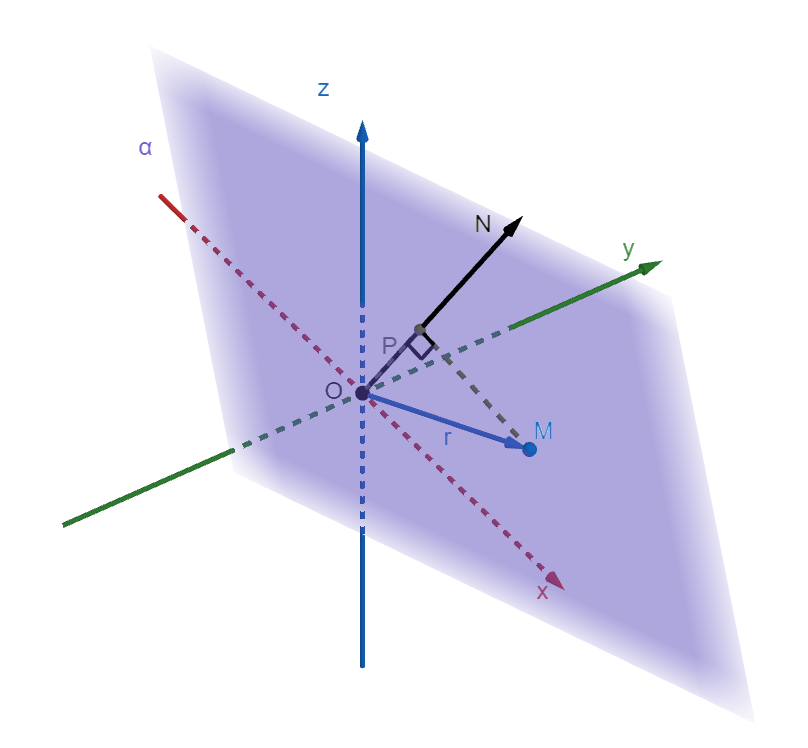
\includegraphics[width=5.5cm]{Images/Chapter_1/2-2-14.png}
        \end{center}
        \(O(0, 0, 0) \notin L\)

        \(P = |O, \alpha| > 0\)

        \(\vec n_0 \perp \alpha\), \(|\vec n_0| = 1\)

        \(\vec n_0\) направлен в сторону \(\alpha\) если его приложить к \(O\)

        \(\vec n_0 = (\cos \alpha, \cos \beta, \cos \gamma)\)

        \(M(x, y, z) \in \alpha\)

        \(P = \proj_{\vec n_0} \vec r \Leftrightarrow\)

        \(\Leftrightarrow\) \fbox{\(\vec r \cdot \vec n_0 - P = 0\)}

        \scriptsize\fbox{\(x \cos \alpha + y \cos \beta + z \cos \gamma - P = 0\)}\normalsize

        \(\alpha: Ax + By + Cz + D = 0\), \(A^2 + B^2 + C^2 \neq 0\)

        \(\vec N = (A, B, C) \perp L \Rightarrow\)

        \(\Rightarrow \vec n_0 = \dfrac{\pm \vec N}{|\vec N|}\)

        \(C > 0: ``+"\)

        \(C < 0: ``-"\)

        \(\cos \alpha = \dfrac{\pm A}{\sqrt{A^2 + B^2 + C^2}}\)

        \(\cos \beta = \dfrac{\pm B}{\sqrt{A^2 + B^2 + C^2}}\)

        \(\cos \gamma = \dfrac{\pm C}{\sqrt{A^2 + B^2 + C^2}}\)

        \(P = \dfrac{\pm D}{\sqrt{A^2 + B^2 + C^2}}\)
         &

        \\
        \hline
        Расстояние от точки до прямой:
        \begin{center}
            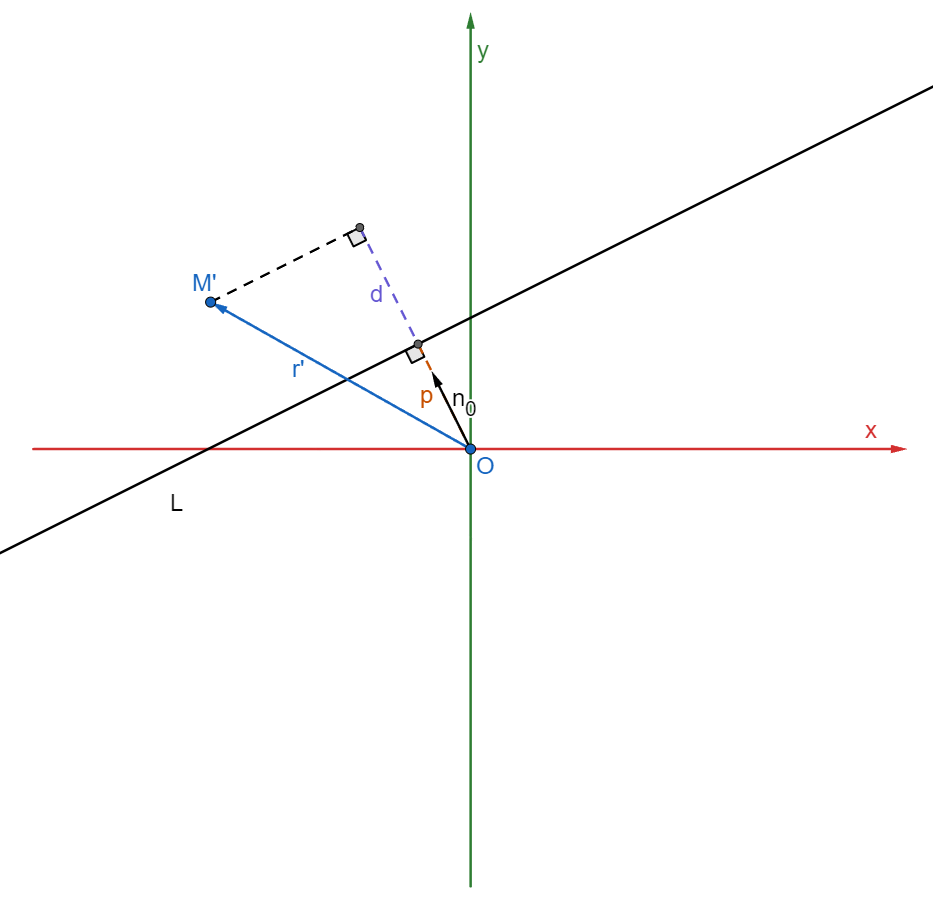
\includegraphics[width=5.5cm]{Images/Chapter_1/2-2-6.png}
        \end{center}
        \(M(x', y')\)

        \(\vec{r'} = \overrightarrow{OM'} = (x', y')\)

        \(L\) задана нормальным уравнением

        \(\proj_{\vec n_0} \vec{r'} - P = \delta\) --- отклонение

        \(\delta > 0\), если \(M'\) и \(O\) лежат по разные стороны от \(L\)

        \(\delta < 0\), если \(M'\) и \(O\) лежат по одну сторону от \(L\)

        \(d = |M', L| = |\delta| = \)

        \(=\) \fbox{\(|\vec{r'} \cdot \vec n_0 - P|\)} \(=\)

        \small\(=\) \fbox{\(|x' \cos \alpha + y' \sin \alpha - P|\)} \(=\)\normalsize

        \(L: Ax + By + C = 0\)

        \fbox{\(d = \dfrac{|Ax' + By' + C|}{\sqrt{A^2 + B^2}}\)}

        \small Работает даже если \(O \in L\)\normalsize
         &
        Расстояние от точки до плоскости:
        \begin{center}
            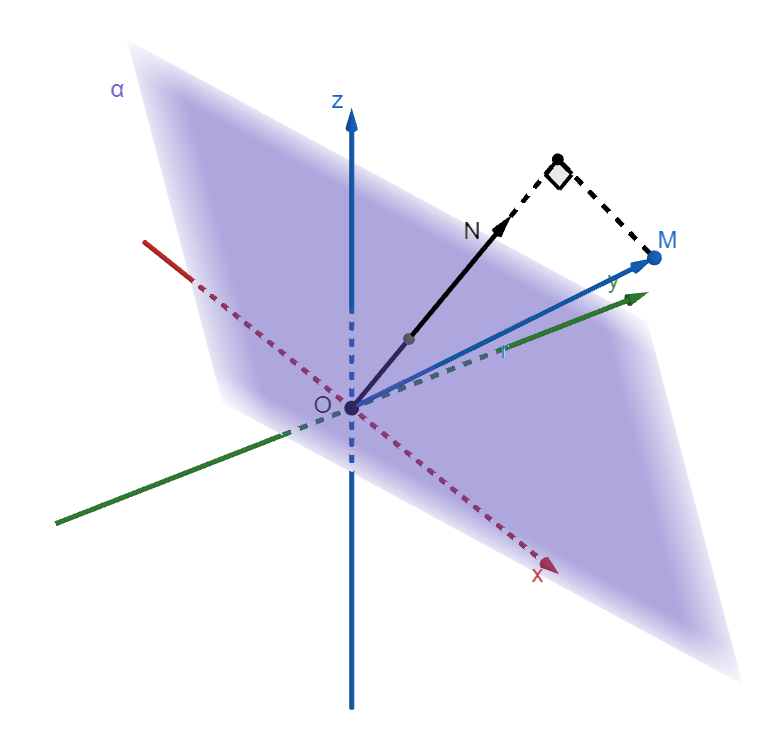
\includegraphics[width=5.5cm]{Images/Chapter_1/2-2-15.png}
        \end{center}
        \(M(x', y', z')\)

        \(\vec{r'} = \overrightarrow{OM'} = (x', y', z')\)

        \(\alpha\) задана нормальным уравнением

        \(\proj_{\vec n_0} \vec{r'} - P = \delta\) --- отклонение

        \(\delta > 0\), если \(M'\) и \(O\) лежат по разные стороны от \(\alpha\)

        \(\delta < 0\), если \(M'\) и \(O\) лежат по одну сторону от \(\alpha\)

        \(d = |M', \alpha| = |\delta| = \)

        \(=\) \fbox{\(|\vec{r'} \cdot \vec n_0 - P|\)} \(=\)

        \scriptsize\(=\) \fbox{\(|x' \cos \alpha + y' \cos \beta + z' \cos \gamma - P|\)} \(=\)\normalsize

        \(\alpha: Ax + By + Cz + D = 0\)

        \small\fbox{\(d = \dfrac{|Ax' + By' + Cz' + D|}{\sqrt{A^2 + B^2 + C^2}}\)}\normalsize

        \small Работает даже если \(O \in \alpha\)\normalsize
         &
        Расстояние от точки до прямой:
        \begin{center}
            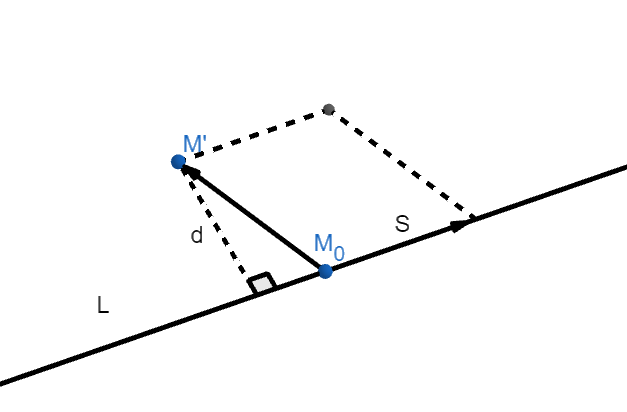
\includegraphics[width=5.5cm]{Images/Chapter_1/2-2-21.png}
        \end{center}
        \(d = |M', L| = \)

        \small\(= h(\)параллелограмма, построенного на \(\vec S\) и \(\overrightarrow{M_0 M'}) =\)\normalsize

        \(=\) \fbox{\(\dfrac{|\vec S \times \overrightarrow{M_0 M'}|}{|\vec S|}\)}
        \\
        \hline
        Полярное уравнение:
        \begin{center}
            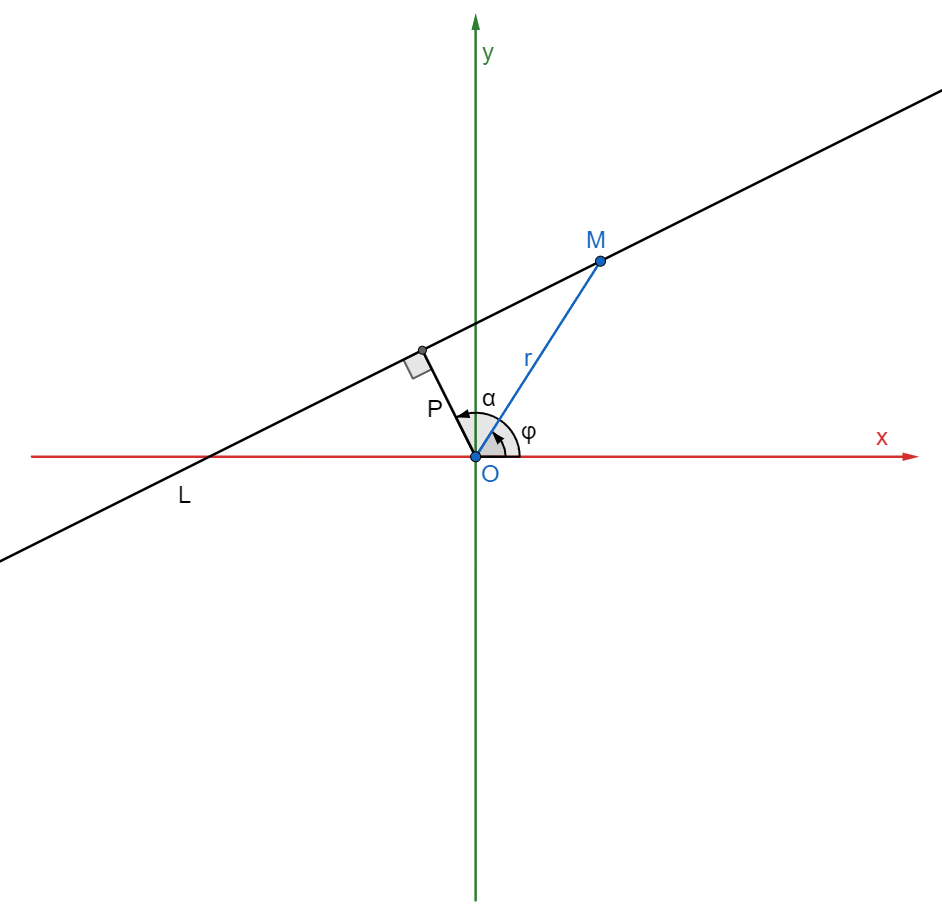
\includegraphics[width=5.5cm]{Images/Chapter_1/2-2-7.png}
        \end{center}
        \(O(0, 0) \notin L\)

        (Если \(O \in L\), то \(L\) распадается на 2 луча и точку \(O\))

        \(M(x, y) \in L\)

        \((x, y) \leftrightarrow (\varphi, r)\):

        \(
        \begin{cases}
            x = r \cos \varphi \\
            y = r \sin \varphi
        \end{cases}
        \)

        \(L\) задана нормальным уравнением:

        \small\(x \cos \alpha + y \sin \alpha - P = 0 \Leftrightarrow\)

        \scriptsize\(\Leftrightarrow r \cos \varphi \cos \alpha - r \sin \varphi \sin \alpha - P = 0 \Leftrightarrow\)

        \small\(\Leftrightarrow r \cos (\varphi - \alpha) - P = 0 \Leftrightarrow\)\normalsize

        \fbox{\(r = \dfrac{P}{\cos(\varphi - \alpha)}\)}

        \(r > 0\)

        \(P > 0\)

        \(\cos(\varphi - \alpha) > 0\)
         &
        \multicolumn{2}{p{11cm}}{

        Взаимное расположение прямой и плоскости в пространстве:

        \(\alpha: Ax + By + Cz + D = 0\), \(A^2 + B^2 + C^2 \neq 0\)

        \(L: \vec S = (l, m, n), M(x_0, y_0, z_0)\)

        \textbullet \(
        \left[\begin{array}{ll}
                  L \parallel \alpha \\
                  L \subset \alpha
              \end{array}\right .\)
        \(\Leftrightarrow \vec S \perp \vec N \Leftrightarrow \vec S \cdot \vec N = 0 \Leftrightarrow\)

        \(\)

        \(\Leftrightarrow Al + Bm + Cn = 0\)

        \textbullet \(L \subset \alpha \Leftrightarrow\)
        \(\begin{cases}
              \vec S \cdot \vec N = 0 \\
              M_0 \in \alpha
          \end{cases} \Leftrightarrow\)

        \(\Leftrightarrow
        \begin{cases}
            Al + Bm + Cn = 0 \\
            Ax_0 + By_0 + Cz_0 + D = 0
        \end{cases}\)

        \textbullet \(
        \begin{cases}
            L \parallel \alpha \\
            L \not\subset \alpha
        \end{cases} \Leftrightarrow
        \begin{cases}
            Al + Bm + Cn = 0 \\
            Ax_0 + By_0 + Cz_0 + D \neq 0
        \end{cases}\)

        \textbullet \(L \cap \alpha = Q\):
        \begin{center}
            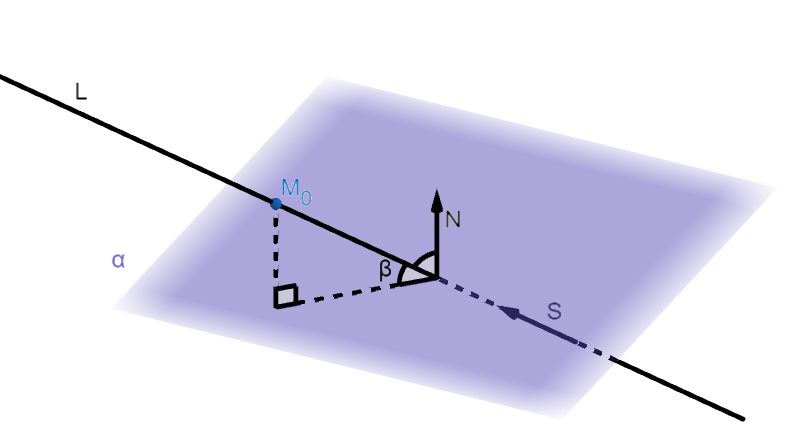
\includegraphics[width=7cm]{Images/Chapter_1/2-2-22.png}
        \end{center}
        \(Q(x_Q, y_Q, z_Q) \in L \Leftrightarrow
        \begin{cases}
            x_Q = x_0 + l t_Q \\
            y_Q = y_0 + m t_Q \\
            z_Q = z_0 + n t_Q
        \end{cases}\)

        \small\(Q \in \alpha \Leftrightarrow A(x_0 + l t_Q) + B(y_0 + m t_Q) + C(z_0 + n t_Q) + D = 0\)\normalsize

        \(\Leftrightarrow\)\fbox{\(t_Q = - \dfrac{Ax_0 + By_0 + Cz_0 + D}{Al + Bm + Cn}\)}

        \(\sin\angle(L, \alpha) = \cos(90^\circ - \angle(L, \alpha)) = \cos\angle(\vec N, \vec S) = \)

        \(=\) \fbox{\(\dfrac{\vec N \cdot \vec S}{|\vec N||\vec S|}\)}
        }\vline
        \\
        \hline
        Взаимное расположение прямых на плоскости:
        \textbullet \(L_1 \parallel L_2\):
        \begin{center}
            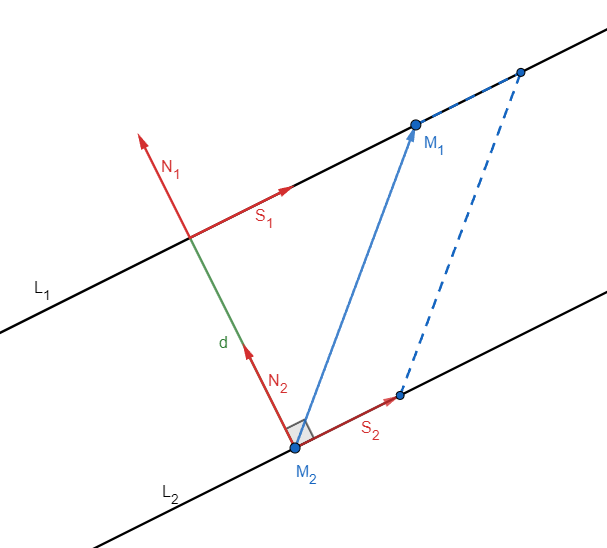
\includegraphics[width=5.5cm]{Images/Chapter_1/2-2-8.png}
        \end{center}
        \(L_1 \parallel L_2 \Leftrightarrow\)

        \(\Leftrightarrow \vec N_1 \parallel \vec N_2 \Leftrightarrow\)

        \(\Leftrightarrow \vec S_1 \parallel \vec S_2 \Leftrightarrow\)

        \(\Leftrightarrow\)\fbox{\(\dfrac{A_1}{A_2} = \dfrac{B_1}{B_2} \Leftrightarrow \dfrac{m_1}{m_2} = \dfrac{n_1}{n_2}\)}

        \(d = |L_1, L_2|\)(парам. ур.)\(=\)

        \small\(= h(\)параллелограмма, построенного на \(\vec S_2\) и \(\overrightarrow{M_2 M_1}) =\)\normalsize

        \(=\) \fbox{\(\dfrac{|\vec S_2 \times \overrightarrow{M_2 M_1}|}{|\vec S_2|}\)} \(=\)

        \(= |M_1, L_2|\)

        \textbullet \(L_1 = L_2 \Leftrightarrow\)

        \(\Leftrightarrow\)\fbox{\(\dfrac{A_1}{A_2} = \dfrac{B_1}{B_2} = \dfrac{C_1}{C_2}\)}

        \textbullet \(L_1 \cap L_2 = Q\):
        \begin{center}
            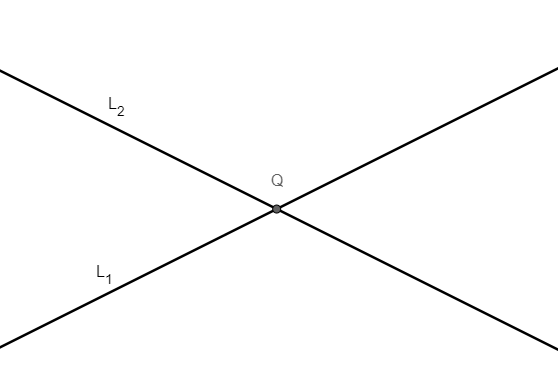
\includegraphics[width=5.5cm]{Images/Chapter_1/2-2-9.png}
        \end{center}
        \(L_1 \cap L_2 \Leftrightarrow \dfrac{A_1}{A_2} \neq \dfrac{B_1}{B_2}\)

        \small\(Q:
        \begin{cases}
            A_1 x + B_1 y + C_1 = 0 \\
            A_2 x + B_2 y + C_2 = 0
        \end{cases}
        \)\normalsize

        \(\Delta =
        \begin{vmatrix}
            A_1 & B_1 \\
            A_2 & B_2
        \end{vmatrix} =\)

        \(= A_1 B_2 - A_2 B_1 \neq 0 \Leftrightarrow\)

        \(\Leftrightarrow \exists ! \; Q\)
         &
        Взаимное расположение плоскостей в пространстве:

        \textbullet \(\alpha_1 \parallel \alpha_2\):
        \begin{center}
            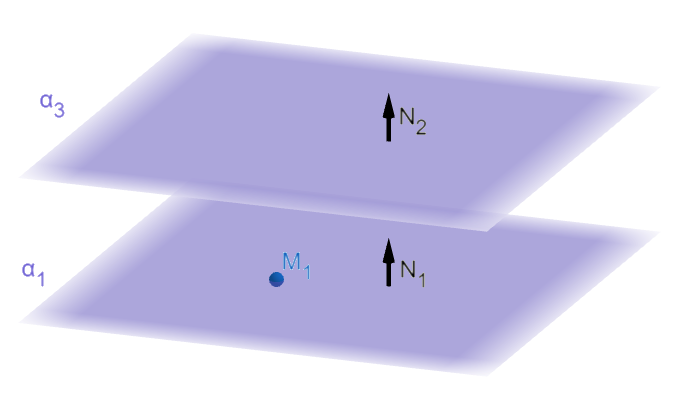
\includegraphics[width=5.5cm]{Images/Chapter_1/2-2-16.png}
        \end{center}
        \(\alpha_1 \parallel \alpha_2 \Leftrightarrow \vec N_1 \parallel \vec N_2 \Leftrightarrow\)

        \(\Leftrightarrow\) \fbox{\(\dfrac{A_1}{A_2} = \dfrac{B_1}{B_2} = \dfrac{C_1}{C_2}\)}

        \(d = |\alpha_1, \alpha_2|\)

        \(M_1 \in \alpha_1 \Rightarrow d = |M_1, \alpha_2|\)

        \(\alpha_1, \alpha_2\) заданы нормальным уравнением:

        \small\(d =
        \begin{cases}
            |P_1 - P_2|, \vec n_{0_1} = \vec n_{0_2} \\
            P_1 + P_2, \vec n_{0_1} = -\vec n_{0_2}  \\
        \end{cases}\)\normalsize

        \textbullet \(\alpha_1 = \alpha_2\):

        \fbox{\(\dfrac{A_1}{A_2} = \dfrac{B_1}{B_2} = \dfrac{C_1}{C_2} = \dfrac{D_1}{D_2}\)}

        \textbullet \(\alpha_1 \cap \alpha_2 = L\):
        \begin{center}
            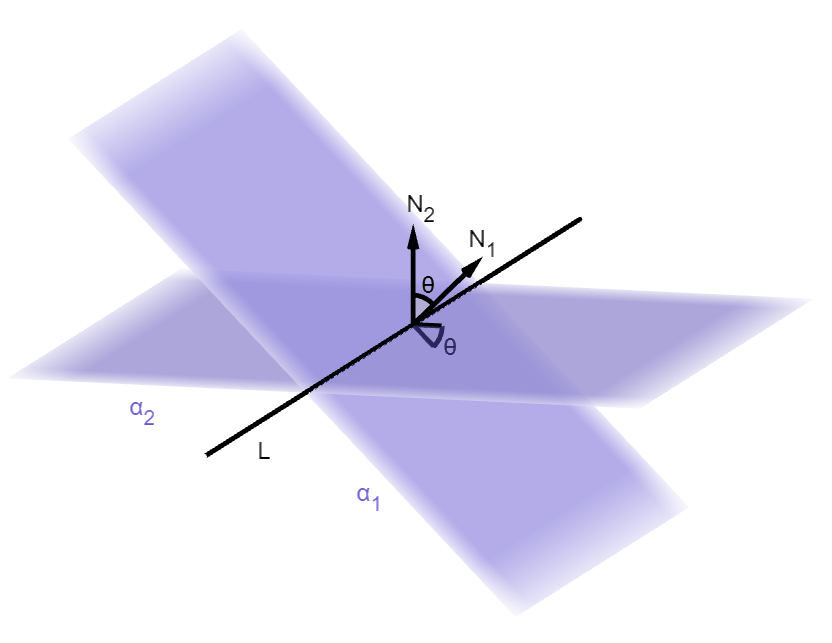
\includegraphics[width=5.5cm]{Images/Chapter_1/2-2-17.png}
        \end{center}
        \small\(L:\)

        \(\begin{cases}
              A_1 x + B_1 y + C_1 z + D_1 = 0 \\
              A_2 x + B_2 y + C_2 z + D_2 = 0
          \end{cases}\)\normalsize

        \(\Rightarrow
        \left[
        \begin{array}{lll}
            \dfrac{A_1}{A_2} \neq \dfrac{B_1}{B_2} \\
            \dfrac{B_1}{B_2} \neq \dfrac{C_1}{C_2} \\
            \dfrac{A_1}{A_2} \neq \dfrac{C_1}{C_2}
        \end{array}
        \right .\)

        \(\theta = \angle(\alpha_1, \alpha_2)\)

        \(|\cos\theta| = \dfrac{|\vec N_1 \cdot \vec N_2|}{|\vec N_1||\vec N_2|}\)
         &
        Взаимное расположение прямых в пространстве:

        \small\textbullet \(\left[
        \begin{array}{ll}
            L_1 \parallel L_2 \\
            L_1 = L_2
        \end{array}\right .\Leftrightarrow \vec S_1 \parallel \vec S_2 \Leftrightarrow\)\normalsize

        \(\Leftrightarrow\) \fbox{\(\dfrac{l_1}{l_2} = \dfrac{m_1}{m_2} = \dfrac{n_1}{n_2}\)}

        \small\textbullet\(L_1 = L_2 \Leftrightarrow
        \begin{cases}
            \vec S_1 \parallel \vec S_2 \\
            M_1 \in L_2
        \end{cases} \Leftrightarrow\)\normalsize

        \(\Leftrightarrow \vec S_1 \parallel \vec S_2 \parallel \overrightarrow{M_1 M_2} \Leftrightarrow\)

        \scriptsize\fbox{\(\Leftrightarrow
            \begin{cases}
                \dfrac{l_1}{l_2} = \dfrac{m_1}{m_2} = \dfrac{n_1}{n_2} \\
                \dfrac{l_1}{x_1 - x_2} = \dfrac{m_1}{y_1 - y_2} = \dfrac{n_1}{z_1 - z_2}
            \end{cases}\)}\normalsize

        \textbullet \(
        \begin{cases}
            L_1 \parallel L_2 \\
            L_1 \neq L_2
        \end{cases} \Leftrightarrow\)

        \(\Leftrightarrow
        \begin{cases}
            \vec S_1 \parallel \vec S_2 \\
            M_1 \notin L_2
        \end{cases}\Leftrightarrow\)

        \(\Leftrightarrow
        \begin{cases}
            \vec S_1 \parallel \vec S_2 \\
            \vec S_1 \nparallel \overrightarrow{M_1 M_2}
        \end{cases}\)

        \(d = |L_1, L_2| = |M_1, L_2| =\)

        \(= \dfrac{|\vec S \times \overrightarrow{M_1 M_2}|}{|\vec S|}\)

        \textbullet\(L_1 \cap L_2 = Q \Leftrightarrow\)

        \(\Leftrightarrow\)\fbox{\(
            \begin{cases}
                \vec S_1 \nparallel \vec S_2 \\
                \vec S_1 \vec S_2 \overrightarrow{M_1 M_2} = 0
            \end{cases}\)}

        \(\cos\angle(L_1, L_2) = \dfrac{\vec S_1 \cdot \vec S_2}{|\vec S_1||\vec S_2|}\)

        \textbullet \(L_1 \skewed L_2:\)

        \begin{center}
            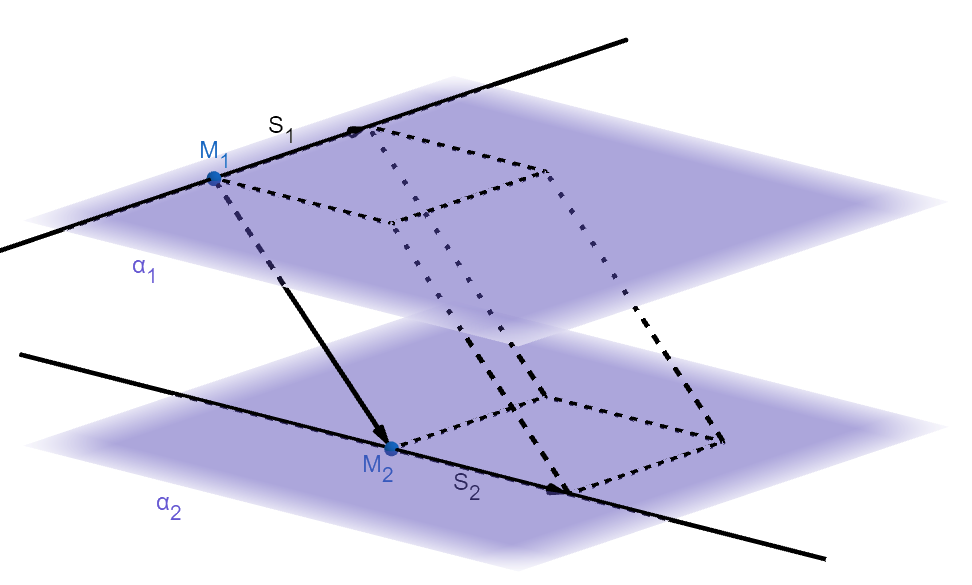
\includegraphics[width=5.5cm]{Images/Chapter_1/2-2-23.png}
        \end{center}

        \(\vec S_1 \vec S_2 \overrightarrow{M_1 M_2} \neq 0 \Rightarrow\)

        \(\Rightarrow \exists \alpha_1, \alpha_2:
        \begin{cases}
            \alpha_1 \parallel \alpha_2 \\
            L_1 \subset \alpha_1        \\
            L_2 \subset \alpha_2
        \end{cases}\)
        \\ & &
        \(|L_1, L_2| = |\alpha_1, \alpha_2| = h(\)параллелепипед, построенный на \(\vec S_1, \vec S_2, \overrightarrow{M_1 M_2}) = \)

        \(=\)\fbox{\(\dfrac{|\vec S_1 \vec S_2 \overrightarrow{M_1 M_2}|}{|\vec S_1 \times \vec S_2|}\)}

        \begin{center}
            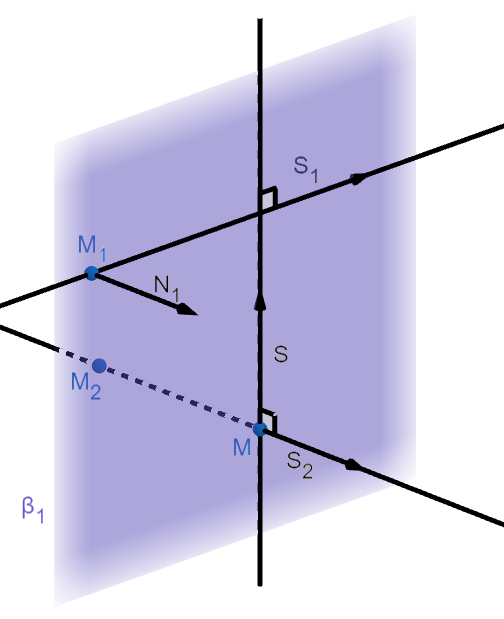
\includegraphics[width=5.5cm]{Images/Chapter_1/2-2-24.png}
        \end{center}
        \(L(M, \vec S):
        \begin{cases}
            L \perp L_1 \\
            L \perp L_2
        \end{cases}\)

        \(\vec S = \vec S_1 \times \vec S_2\)

        \(\beta_1(\vec S_1, \vec S, M_1) \Rightarrow\)

        \(\Rightarrow\)\fbox{\(M = L_2 \cap \beta_1\)}

        \(\vec N_1 = \vec S_1 \times \vec S =\)

        \(= \vec S_1 \times (\vec S_1 \times \vec S_2)\)
        \\
        \hline
    \end{longtable}
\end{center}


\subsection{Проекция точки на плоскость и прямую}
\begin{center}
    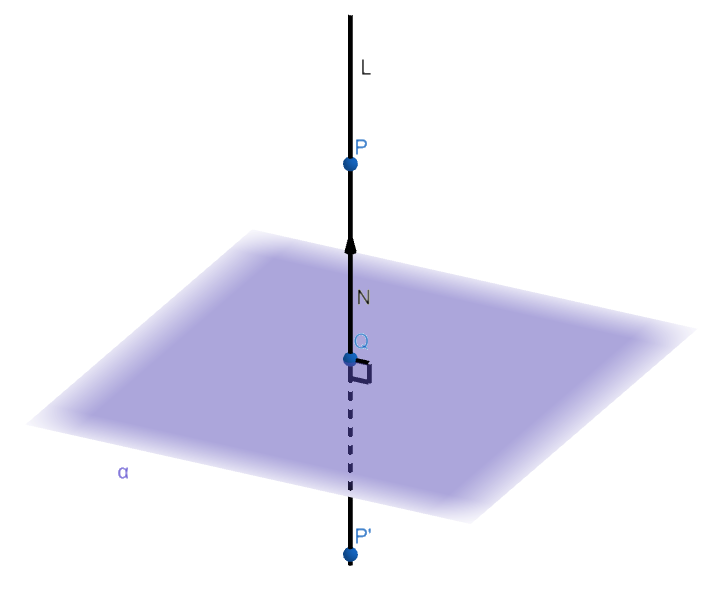
\includegraphics[height=7cm]{Images/Chapter_1/2-3-1.png}
\end{center}
\(PQ \perp \alpha\), \(Q \in \alpha\)

\(\alpha: Ax + By + Cz + D = 0\), \(\vec N = (A, B, C)\)

\(P(P_1, P_2, P_3)\)

\(L(P, \vec N):
\begin{cases}
    x = P_1 + t A \\
    y = P_2 + t B \\
    z = P_3 + t C
\end{cases} \Rightarrow Q = L \cap \alpha \Rightarrow\)

\(\Rightarrow A(P_1 + t_Q A) + B(P_2 + t_Q B) + C(P_3 + t_Q C) + D = 0 \Rightarrow\)\fbox{\(t_Q = - \dfrac{AP_1 + BP_2 + CP_3 + D}{A^2 + B^2 + C^2}\)}

\(P'\) --- отражение \(P\) относительно \(\alpha \Rightarrow P' = 2Q - P\)
\begin{center}
    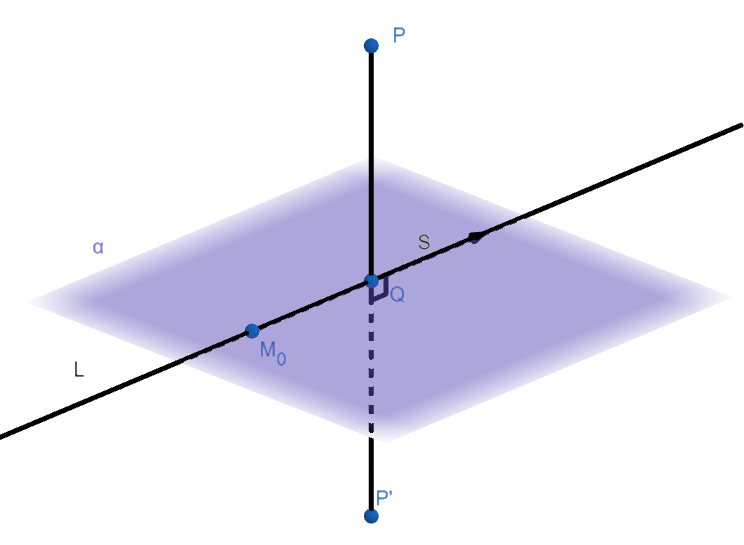
\includegraphics[height=7cm]{Images/Chapter_1/2-3-2.png}
\end{center}
\(PQ \perp L(M_0, \vec S = (l, m, n))\), \(Q \in L\)

\(P = (P_1, P_2, P_3)\)

\(\alpha(P, \vec S): l(x - P_1) + m(y - P_2) + n(z - P_3) = 0\)
\(L:
\begin{cases}
    x = x_0 + t l \\
    y = y_0 + t m \\
    z = z_0 + t n
\end{cases}\)

\(Q = \alpha \cap L \Rightarrow l((x_0 + t_Q l) - P_1) + m((y_0 + t_Q m) - P_2) + n((z_0 + t_Q n) - P_3) = 0\)

Находим из этого \(t_Q\) и подставляем в уравнение \(L\).

\(P'\) --- отражение \(P\) относительно \(L \Rightarrow P' = 2Q - P\)


\section{Кривые второго порядка (КВП)}
\subsection{Канонические уравнения КВП}
Кривая второго порядка --- множество точек на плоскости, декартовы координаты которых удовлетворяет алгебраическому уравнению 2-го порядка:

\(a_{11} x^2 + 2 a_{12} xy + a_{22} y^2 + 2 a_1 x + 2 a_2 y + a_0 = 0\), \((a_{11}^2 + a_{12}^2 + a_{22}^2 \neq 0)\)

КВП делятся на 2 вида:
\begin{enumerate}
    \item Невырожденные:
          \begin{itemize}
              \item Эллипс
              \item Парабола
              \item Гипербола
          \end{itemize}
    \item Вырожденные:
          \begin{itemize}
              \item Пара пересекающихся прямых
              \item Пара параллельных прямых
              \item Пара совпадающих прямых
              \item Точка
              \item Пустое множество
          \end{itemize}
\end{enumerate}

\begin{center}
    \begin{longtable}{|p{2.5cm}|p{4.5cm}|p{4.5cm}|p{4.5cm}|}
        \hline
         &
        Эллипс
         &
        Гипербола
         &
        Парабола
        \\
        \hline
        Опр. 1
         &
        ГМТ на плоскости, таких, что сумма расстояний до двух фиксированных точек плоскости --- величина постоянная и равная \(2a\).
        \begin{center}
            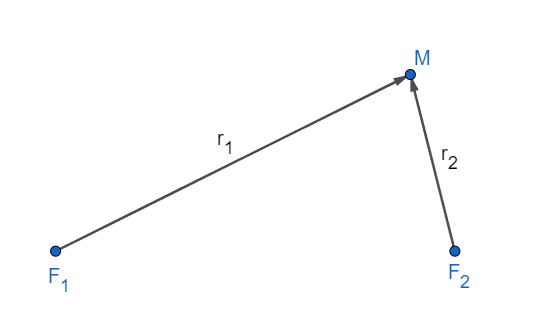
\includegraphics[width=4.5cm]{Images/Chapter_1/3-1-1.png}
        \end{center}
        \(r_1 + r_2 = 2a = \mathbf{const}\)
         &
        ГМТ на плоскости, таких, что модуль разности расстояний до двух фиксированных точек плоскости --- величина постоянная и равная \(2a\).
        \begin{center}
            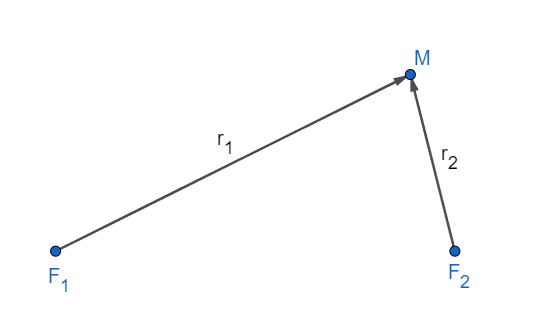
\includegraphics[width=4.5cm]{Images/Chapter_1/3-1-1.png}
        \end{center}
        \(|r_1 - r_2| = 2a = \mathbf{const}\)
         &
        ГМТ на плоскости, таких, что расстояние до фиксированной точки плоскости равно расстоянию до фиксированной прямой.
        \begin{center}
            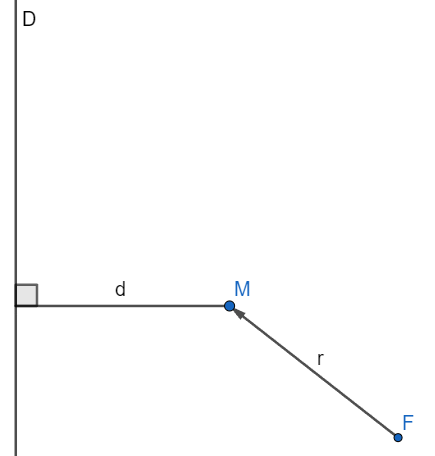
\includegraphics[width=4.5cm]{Images/Chapter_1/3-1-2.png}
        \end{center}
        \(r = d\)
        \\
        \hline
        Уравнение в ДСК
         &
        \begin{center}
            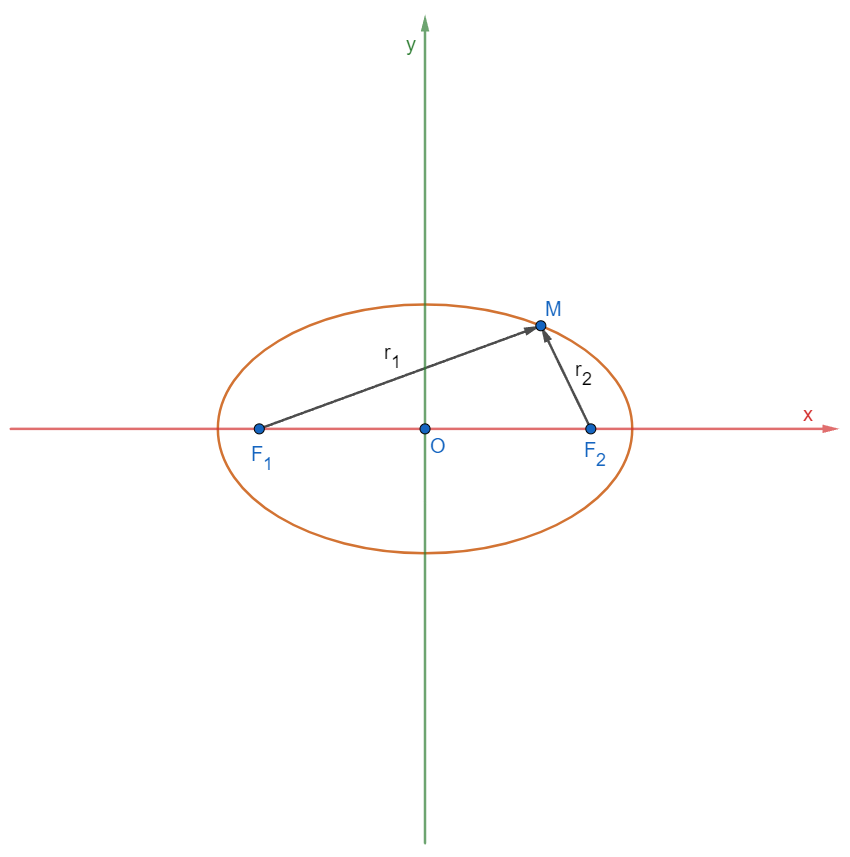
\includegraphics[width=4.5cm]{Images/Chapter_1/3-1-3.png}
        \end{center}
        \(F_{1, 2}\) --- фокусы

        \(F_1(-c, 0)\), \(F_2(c, 0)\)

        \fbox{\(\dfrac{x^2}{a^2} + \dfrac{y^2}{b^2} = 1\)}

        \(a^2 = b^2 + c^2\), \(a > c\)

        \(r_1, r_2\) --- фокальные радиусы

        \(a\) --- большая полуось

        \(b\) --- малая полуось
         &
        \begin{center}
            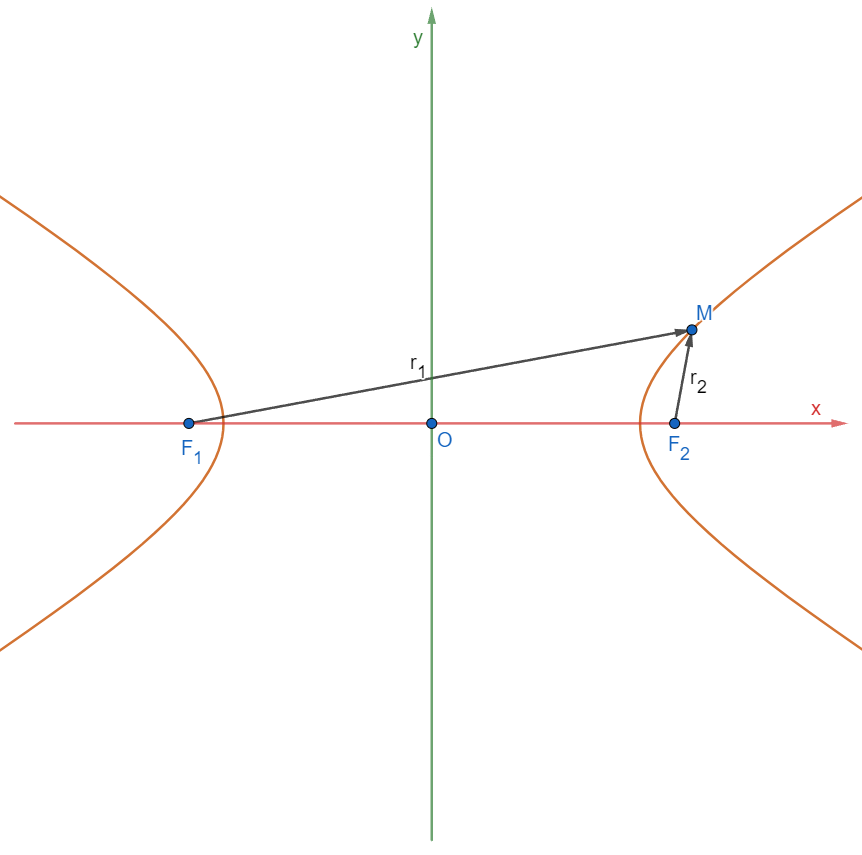
\includegraphics[width=4.5cm]{Images/Chapter_1/3-1-4.png}
        \end{center}
        \(F_{1, 2}\) --- фокусы

        \(F_1(-c, 0)\), \(F_2(c, 0)\)

        \fbox{\(\dfrac{x^2}{a^2} - \dfrac{y^2}{b^2} = 1\)}

        \(c^2 = a^2 + b^2\), \(a < c\)

        \(r_1, r_2\) --- фокальные радиусы

        \(a\) --- действительная полуось

        \(b\) --- мнимая полуось

        Имеет асимптоты --- \(y = \pm \dfrac{b}{a} x\)

        \(\)
         &
        \begin{center}
            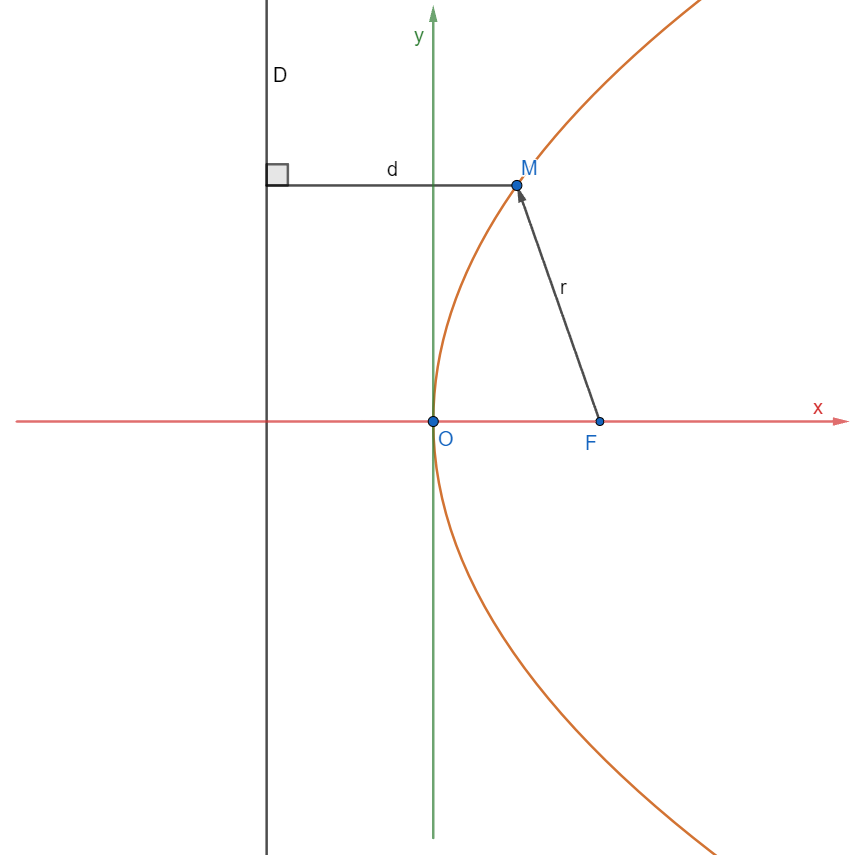
\includegraphics[width=4.5cm]{Images/Chapter_1/3-1-5.png}
        \end{center}
        \(F\) --- фокус, \(D\) --- директриса

        \(F\left(\dfrac{p}{2}, 0\right)\), \(D: x = -\dfrac{p}{2}\)

        \fbox{\(y^2 = 2px\)}

        \(p = |F, D|\)

        \(p\) --- фокальный параметр
        \\
        \hline
        \(\varepsilon\) --- Эксцентриситет
         &
        \(\varepsilon = \dfrac{c}{a} < 1\)
         &
        \(\varepsilon = \dfrac{c}{a} > 1\)
         &
        \(\varepsilon = 1\)
        \\
        \hline
        \(r_{1, 2}\) --- фокальные радиусы
         &
        \(r_{1, 2} = a \pm \varepsilon x\)

        \(M(x, y) \in\) эллипсу
         &
        Правая ветвь:

        \(r_{1, 2} = \varepsilon x \pm a\)

        Левая ветвь:

        \(r_{1, 2} = -\varepsilon x \mp a\)

        \(M(x, y) \in\) гиперболе
         &
        \(r = x + \dfrac{p}{2}\)
        \\
        \hline
        Директрисы
         &
        \begin{center}
            \includegraphics[width=4.5cm]{Images/Chapter_1/3-1-6.png}
        \end{center}
        \(D_{1, 2}: x = \mp \dfrac{a}{\varepsilon}\)

        \(\dfrac{r_1}{d_1} = \dfrac{r_2}{d_2} = \varepsilon = \dfrac{r}{d}\)
         &
        \begin{center}
            \includegraphics[width=4.5cm]{Images/Chapter_1/3-1-7.png}
        \end{center}
        \(D_{1, 2}: x = \mp \dfrac{a}{\varepsilon}\)

        \(\dfrac{r_1}{d_1} = \dfrac{r_2}{d_2} = \varepsilon = \dfrac{r}{d}\)
         &
        \(\dfrac{r}{d} = 1 = \varepsilon\)
        \\
        \hline
        Опр. 2
         &
        ГМТ на плоскости, таких, что отношение расстояния до фиксированной точки плоскости к расстоянию до прямой --- величина постоянная и меньшая единицы.

        \(\varepsilon = \mathbf{const} = \dfrac{r}{d} < 1\)
        \begin{center}
            \includegraphics[width=4.5cm]{Images/Chapter_1/3-1-8.png}
        \end{center}
         &
        ГМТ на плоскости, таких, что отношение расстояния до фиксированной точки плоскости к расстоянию до прямой --- величина постоянная и большая единицы.

        \(\varepsilon = \mathbf{const} = \dfrac{r}{d} > 1\)
        \begin{center}
            \includegraphics[width=4.5cm]{Images/Chapter_1/3-1-9.png}
        \end{center}
         &
        ГМТ на плоскости, таких, что отношение расстояния до фиксированной точки плоскости к расстоянию до прямой --- величина постоянная и равная единице.

        \(\varepsilon = \mathbf{const} = \dfrac{r}{d} = 1\)
        \begin{center}
            \includegraphics[width=4.5cm]{Images/Chapter_1/3-1-2.png}
        \end{center}
        \\
        \hline
        Полярное уравнение
         &
        \begin{center}
            \includegraphics[width=4.5cm]{Images/Chapter_1/3-1-10.png}
        \end{center}
        Начало ПСК в одном из фокусов, ось направлена в сторону соответствующей директрисы.

        \(r = \dfrac{P}{1 + \varepsilon \cos\varphi}\)

        \(P\) --- фокальный параметр.

        \(P = \varepsilon \cdot q = \dfrac{b^2}{a}\)

        \(q = |F, D| = \dfrac{a}{\varepsilon} - c\)

        \(P\) --- Длина перпендикуляра от \(F\) до эллипса

        Директрисы:

        \(r = \dfrac{\pm \dfrac{a}{\varepsilon} - c}{\cos\varphi}\)

        Если ось направлена в противоположную сторону, то меняем знак косинуса.
         &
        \begin{center}
            \includegraphics[width=4.5cm]{Images/Chapter_1/3-1-11.png}
        \end{center}
        Начало ПСК в одном из фокусов, ось направлена в сторону соответствующей директрисы.

        \(r = \dfrac{\pm P}{1 \pm \varepsilon \cos\varphi}\)

        Ветвь, более близкая к фокусу: \(``+"\)

        Ветвь, более далёкая от фокуса: \(``-"\)

        \(P\) --- фокальный параметр.

        \(P = \varepsilon \cdot q = \dfrac{b^2}{a}\)

        \(q = |F, D| = c - \dfrac{a}{\varepsilon}\)

        \(P\) --- Длина перпендикуляра от \(F\) до гиперболы.

        Директрисы:

        \(r = \dfrac{\pm \dfrac{a}{\varepsilon} + c}{\cos\varphi}\)

        Если ось направлена в противоположную сторону, то меняем знак косинуса.
         &
        \begin{center}
            \includegraphics[width=4.5cm]{Images/Chapter_1/3-1-12.png}
        \end{center}
        Начало ПСК в фокусе, ось направлена в сторону директрисы.

        \(r = \dfrac{P}{1 + \varepsilon \cos\varphi} = \)

        \(= \dfrac{P}{1 + \cos\varphi}\)

        \(P\) --- Длина перпендикуляра от \(F\) до параболы

        Если ось направлена в противоположную сторону, то меняем знак косинуса.
        \\
        \hline
        Касательные
         &
        \begin{center}
            \includegraphics[width=4.5cm]{Images/Chapter_1/3-1-13.png}
        \end{center}
        \(M(x_0, y_0) \in\) эллипсу

        \(\dfrac{x x_0}{a^2} + \dfrac{y y_0}{b^2} = 1\)
         &
        \begin{center}
            \includegraphics[width=4.5cm]{Images/Chapter_1/3-1-14.png}
        \end{center}
        \(M(x_0, y_0) \in\) гиперболе

        \(\dfrac{x x_0}{a^2} - \dfrac{y y_0}{b^2} = 1\)
         &
        \begin{center}
            \includegraphics[width=4.5cm]{Images/Chapter_1/3-1-15.png}
        \end{center}
        \(M(x_0, y_0) \in\) параболе

        \(y y_0 = P(x + x_0)\)
        \\
        \hline
        Оптические свойства
         &
        \begin{center}
            \includegraphics[width=4.5cm]{Images/Chapter_1/3-1-16.png}
        \end{center}
        Любой луч, вышедший из одного фокуса, отразившись, пройдёт через другой фокус.
         &
        \begin{center}
            \includegraphics[width=4.5cm]{Images/Chapter_1/3-1-17.png}
        \end{center}
        Любой луч, вышедший из одного фокуса, отразившись, пройдёт по прямой, проходящей через другой фокус.
         &
        \begin{center}
            \includegraphics[width=4.5cm]{Images/Chapter_1/3-1-18.png}
        \end{center}
        Любой луч, вышедший из фокуса, отразившись, пройдёт по прямой, параллельной оси параболы.
        \\
        \hline
        Другие свойства
         &
        \begin{center}
            \includegraphics[width=4.5cm]{Images/Chapter_1/3-1-19.png}
        \end{center}
        \(\dfrac{MN}{M'N} = \dfrac{b}{a}\)

        Любой эллипс --- сжатая по какой-то оси окружность.
         &
        \begin{center}
            \includegraphics[width=4.5cm]{Images/Chapter_1/3-1-20.png}
        \end{center}
        \(\dfrac{y^2}{b^2} - \dfrac{x^2}{a^2} = 1\) --- сопряжённая гипербола. Имеет те же асимптоты.
         &

        \\
        \hline
    \end{longtable}
\end{center}
Доказательство свойств (на примере гиперболы, эллипс доказывается полностью аналогично):
\begin{itemize}
    \item Каноническое уравнение

          По определению: \(|r_1 - r_2| = 2a\)

          \(F_1(-c, 0)\), \(F_2(c, 0)\), \(c > a\)

          \(r_1 = \sqrt{(x + c)^2 + y^2}\), \(r_2 = \sqrt{(x - c)^2 + y^2}\)

          Пусть \(r_1 > r_2\) (правая ветвь) \(\Rightarrow r_1 = 2a + r_2 \Rightarrow r_1^2 = 4a^2 + 4ar_2 + r_2^2 \Rightarrow\)

          \(\Rightarrow (x + c)^2 + y^2 = 4a^2 + 4ar_2 + (x - c)^2 + y^2 \Rightarrow xc = a^2 + ar_2 \Rightarrow r_2 = \dfrac{xc}{a} - a\)

          \(\varepsilon = \dfrac{c}{a} \Rightarrow\) \fbox{\(r_2 = x \varepsilon - a\)} --- зависимость фокального радиуса от \(x\)

          \(r_2^2 = (x - c)^2 + y^2 \Rightarrow (x - c)^2 + y^2 = \dfrac{x^2 c^2}{a^2} - 2xc + a^2 \Rightarrow x^2\left(1 - \dfrac{c^2}{a^2}\right) + y^2 = a^2 - c^2 \Rightarrow\)

          \(\Rightarrow \dfrac{x^2(a^2 - c^2)}{a^2} + y^2 = a^2 - c^2 \Rightarrow \dfrac{x^2}{a^2} - \dfrac{y^2}{c^2 - a^2} = 1 \Rightarrow\) \fbox{\(\dfrac{x^2}{a^2} - \dfrac{y^2}{b^2} = 1\)} \(Q.E.D.\)

          Из \(r_2 = -2a + r_1\) аналогично можно получить \(r_1 = x \varepsilon + a\). Значит \fbox{\(r_{1, 2} = x \varepsilon \pm a\)}

          Если \(r_1 < r_2\) (левая ветвь): \fbox{\(r_{1, 2} = -x \varepsilon \mp a\)}

    \item Директрисы:

          \(D_2: x = \pm \dfrac{a}{\varepsilon}\), \(d_2 = |M, D_2| = \left|x - \dfrac{a}{\varepsilon}\right|\)

          Правая ветвь: \(r_2 = x \varepsilon - a \Rightarrow \dfrac{r_2}{d_2} = \dfrac{x \varepsilon - a}{x - \dfrac{a}{\varepsilon}} = \varepsilon \dfrac{x - \dfrac{a}{\varepsilon}}{x - \dfrac{a}{\varepsilon}} = \varepsilon\)

          Левая ветвь: \(r_2 = -x \varepsilon + a \Rightarrow \dfrac{r_2}{d_2} = \dfrac{-x \varepsilon + a}{-x + \dfrac{a}{\varepsilon}} = \varepsilon \dfrac{-x + \dfrac{a}{\varepsilon}}{-x + \dfrac{a}{\varepsilon}} = \varepsilon\)

          \(\dfrac{r_2}{d_2} = \varepsilon \Rightarrow D_2\) --- директриса \(Q.E.D.\)

          Для \(r_1\) и \(D_1\) заменить \(x\) на \(-x\)

    \item Определение 2:

          Пусть известно \(Q = |F, D|\) и \(\varepsilon = \dfrac{r}{d} > 1\)

          Проведём ДСК, в которой \(D \parallel Oy\). Давайте найдём параметры канонического уравнения, считая, что \(D: x = \dfrac{a}{\varepsilon}\), а \(F = (c, 0)\).

          \(\begin{rcases}
              c - \dfrac{a}{\varepsilon} = Q \\
              \dfrac{c}{a} = \varepsilon
          \end{rcases} \Rightarrow c = Q + \dfrac{a}{\varepsilon} \Rightarrow a \varepsilon = Q + \dfrac{a}{\varepsilon} \Rightarrow a \left(\varepsilon - \dfrac{1}{\varepsilon}\right) = Q \Rightarrow\) \fbox{\(a = \dfrac{\varepsilon Q}{\varepsilon^2 - 1}\)} \(\Rightarrow\)

          \(\Rightarrow\) \fbox{\(c = \dfrac{\varepsilon^2 Q}{\varepsilon^2 - 1}\)}

          Мы в узнали чему равны \(a\) и \(c\) из известных нам \(\varepsilon\) и \(Q\), значит точки, удовлетворяющие 2-му определению, удовлетворяют \(\dfrac{x^2}{a^2} - \dfrac{y^2}{b^2} = 1\), а \(D\) --- очевидно директриса гиперболы. \(Q.E.D.\)

    \item Асимптоты:

          Найдём \(y(x)\) для I координатной четверти: \(\dfrac{x^2}{a^2} - \dfrac{y^2}{b^2} = 1 \Rightarrow y = b \sqrt{\dfrac{x^2}{a^2} - 1}\)

          Найдём угловой коэффициент асимптоты \(k = \lim\limits_{x \to +\infty}\dfrac{y(x)}{x}\):

          \(k = \lim\limits_{x \to +\infty} \dfrac{b \sqrt{\dfrac{x^2}{a^2} - 1}}{x} = \lim\limits_{x \to +\infty} \dfrac{b x \sqrt{\dfrac{1}{a^2} - \dfrac{1}{x^2}}}{x} = \dfrac{b}{a}\)

          Найдём ординату пересечения асимптоты и оси ординат \(m = \lim\limits_{x \to +\infty}(y(x) - kx)\):

          \(\lim\limits_{x \to +\infty} \left(b \sqrt{\dfrac{x^2}{a^2} - 1} - \dfrac{b}{a}x\right) = b \lim\limits_{x \to +\infty} \left(\sqrt{\dfrac{x^2}{a^2} - 1} - \dfrac{x}{a}\right) =\)

          \(=b \lim\limits_{x \to +\infty} \left(\dfrac{\dfrac{x^2}{a^2} - 1 - \dfrac{x^2}{a^2}}{\sqrt{\dfrac{x^2}{a^2} - 1} + \dfrac{x}{a}} \right) = b \lim\limits_{x \to +\infty} \left(\dfrac{-1}{\sqrt{\dfrac{x^2}{a^2} - 1} + \dfrac{x}{a}} \right) = 0\)

          Значит асимптота: \(y = \dfrac{b}{a} x\)

          По симметрии получаем \(y = \pm \dfrac{b}{a} x\) \(Q.E.D.\)

    \item Полярное уравнение:

          Зададим ПСК\((r, \varphi)\), у которой полюс \(O'= F_2 = (c, 0)\), а ось направлена в сторону \(-x\).

          \(x = c - r \cos \varphi\)

          Правая ветвь: \(r = r_2 = x \varepsilon - a\)

          \(r = \varepsilon(c - r \cos \varphi) - a = \varepsilon c - \varepsilon r \cos \varphi - a \Rightarrow r(1 + \varepsilon \cos \varphi) = \varepsilon c - a = \varepsilon \left(c - \dfrac{a}{\varepsilon}\right) = P \Rightarrow r = \dfrac{P}{1 + \varepsilon \cos \varphi}\)

          Левая ветвь: \(r = r_2 = - x \varepsilon + a\)

          \(r = - \varepsilon(c - r \cos \varphi) + a = - \varepsilon c + \varepsilon r \cos \varphi + a \Rightarrow r(1 - \varepsilon \cos \varphi) = a - \varepsilon c = \varepsilon \left(\dfrac{a}{\varepsilon} - c\right) = -P \Rightarrow r = \dfrac{-P}{1 - \varepsilon \cos \varphi}\)

          Если ось направлена в противоположную сторону, то \(\cos(2 \pi - \varphi) = - \cos \varphi\), и \(\cos \varphi\) в формулы записывается со знаком минус.

          Аналогично, если у ПСК полюс в \(F_1\).

    \item Касательные

          Формула касательной к функции в точке \(M_0(x_0, y_0)\): \(y = f'(x_0)(x - x_0) + y_0\)

          \(\dfrac{x^2}{a^2} - \dfrac{y^2}{b^2} = 1 \Rightarrow \dfrac{x^2}{a^2} - \dfrac{f(x)^2}{b^2} = 1 \Rightarrow (\)Возьмём производную обеих сторон\() \Rightarrow\)

          \(\Rightarrow \dfrac{2x}{a^2} - \dfrac{2 f(x) f'(x)}{b^2} = 0 \Rightarrow \dfrac{2 f(x) f'(x)}{b^2} = \dfrac{2x}{a^2}\)

          Подставим \(x_0\): \(\dfrac{2 f(x_0) f'(x_0)}{b^2} = \dfrac{2x_0}{a^2} \Rightarrow \dfrac{y_0 f'(x_0)}{b^2} = \dfrac{x_0}{a^2} \Rightarrow f'(x_0) = \dfrac{x_0 b^2}{y_0 a^2}\)

          Подставим в формулу для касательной: \(y = \dfrac{x_0 b^2}{y_0 a^2}(x - x_0) + y_0=\)

          \(= \dfrac{x_0 b^2 (x - x_0) + y_0^2 a^2}{y_0 a^2} \Rightarrow\)

          \(\Rightarrow y y_0 a^2 = x x_0 b^2 - x_0^2 b^2 + y_0^2 a^2 \Rightarrow \dfrac{x x_0}{a^2} - \dfrac{y y_0}{b^2} = \dfrac{x_0^2}{a^2} - \dfrac{y_0^2}{b^2} = 1\) \(Q.E.D.\)

    \item Оптические свойства

          Пусть \(M_0(x_0, y_0)\) лежит на гиперболе. Тогда:

          \(\vec r_1 = \overrightarrow{F_1 M_0} = (x_0 + c, y_0)\), \(\vec r_2 = \overrightarrow{F_2 M_0} = (x_0 - c, y_0)\)

          Проверим, что биссектриса между \(\vec r_1\) и \(\vec r_2\) параллельна касательной в точке \(M_0\), то есть перпендикулярна перпендикуляру касательной \(\vec N = \left(\dfrac{x_0}{a^2}, -\dfrac{y_0}{b^2}\right)\).

          Биссектриса между \(\vec r_1\) и \(\vec r_2\): \(|\vec r_1|\vec r_2 + |\vec r_2| \vec r_1 = (\varepsilon x_0 + a) \vec r_2 + (\varepsilon x_0 - a) \vec r_1 =\)

          \(=((x_0 - c)(\varepsilon x_0 + a) + (\varepsilon x_0 - a)(x_0 + c), y_0(\varepsilon x_0 + a) + y_0(\varepsilon x_0 - a)) =\)

          \(= (2\varepsilon x_0^2 - 2ac, 2 \varepsilon x_0 y_0) \sim \left(x_0^2 - \dfrac{ac}{\varepsilon}, x_0 y_0\right)\)

          Скалярно перемножим с \(\vec N\): \(\left(x_0^2 - \dfrac{ac}{\varepsilon}\right)\dfrac{x_0}{a^2} - x_0 y_0 \dfrac{y_0}{b^2} = \dfrac{x_0^3}{a^2} - \dfrac{x_0 c}{\varepsilon a} - \dfrac{x_0 y_0^2}{b^2} =\)

          \(= x_0 \left(\dfrac{x_0^2}{a^2} - \dfrac{y_0^2}{b^2}\right) - x_0 = x_0 - x_0 = 0 \Rightarrow N \perp\) биссектрисе \(Q.E.D.\)
\end{itemize}

\subsection{Приведение КВП к каноническому виду}
\(a_{11} x^2 + 2 a_{12} x y + a_{22} y^2 + 2 a_1 x + 2 a_2 y + a_0 = 0\), \(a_{11}^2 + a_{12}^2 + a_{22}^2 \neq 0\)

Очевидно, что КВП не меняет своего типа при повороте и сдвиге.

\begin{enumerate}
    \item Если \(a_{12} \neq 0\), подберём такой угол поворота \(\alpha\), чтобы в новом уравнении \(a_{12}' = 0\).

          Выразим старые координаты через новые:

          \(x = x' \cos \alpha - y' \sin \alpha\), \(y = x' \sin \alpha + y' \cos \alpha\), \(\alpha \in \left(-\dfrac{\pi}{2}, \dfrac{\pi}{2}\right) \setminus \{0\}\)

          Выразим \(a_{12}'\) через старые коэффициенты, \(\sin \alpha = S_\alpha\) и \(\cos \alpha = C_\alpha\) и приравняем к \(0\):

          \(a_{12} = -2 a_{11} C_\alpha S_\alpha + 2 a_{12} (C_\alpha^2 S_\alpha^2) + 2 a_{22} C_\alpha S_\alpha = 0\)

          \((a_{22} - a_{11}) \tan \alpha + a_{12} (1 - \tan^2 \alpha) = 0\)

          \(\tan^2 \alpha + \dfrac{a_{22} - a_{11}}{a_{12}} \tan \alpha - 1 = 0\) ~--- квадратное уравнение относительно \(\tan \alpha\)

          Дискриминант \(D = \left(\dfrac{a_{22} - a_{11}}{a_{12}}\right) ^ 2 + 4 > 0\) ~--- 2 решения

          По теореме Виета \(\tan \alpha_1 \cdot \tan \alpha_2 = -1 \Rightarrow \alpha_1 \in \left(0, \dfrac{\pi}{2}\right)\), \(\alpha_2 \in \left(-\dfrac{\pi}{2}, 0\right)\), \(\alpha_1 - \alpha_2 = 90^\circ\)

          \(\alpha_{1, 2} = \arctan\left(\dfrac{-\dfrac{a_{22} - a_{11}}{a_{12}} \pm \sqrt{\left(\dfrac{a_{22} - a_{11}}{a_{12}}\right) ^ 2 + 4}}{2}\right)\)

          Начало координат \(O' = O\)

    \item \(a_{11}' x'^2 + a_{22} y'^2 + 2 a_1' x' + 2 a_2' y' + a_0 = 0\)
          Есть два случая:
          \begin{enumerate}
              \item \(\begin{cases}
                        a_{11}' \neq 0 \\
                        a_{22}' \neq 0
                    \end{cases}\)

                    \(a_{11}' x'^2 + 2 a_1' x' = a_{11}' \left(x'^2 + 2 \dfrac{a_1'}{a_{11}'} x'\right) = a_{11}' \left(x' + \dfrac{a_1'}{a_{11}'}\right)^2 - \dfrac{a_1'^2}{a_{11}'} = a_{11}' x''^2 - \dfrac{a_1'^2}{a_{11}'}\)

                    Сделаем сдвиг ДСК:

                    \(x'' = x' + \dfrac{a_1'}{a_{11}'}\)

                    \(y'' = y' + \dfrac{a_2'}{a_{22}'}\)

                    Начало координат \(O''\left(-\dfrac{a_1'}{a_{11}'}, -\dfrac{a_2'}{a_{22}'}\right)\)

                    Получим \(a_{11}' x''^2 + a_{22}' y''^2 + a_0' = 0 \Leftrightarrow a_{11}' x''^2 + a_{22}' y''^2 = -a_0'\)

                    Есть два случая:
                    \begin{enumerate}
                        \item \(a_0' \neq 0\)

                              \(\alpha = \dfrac{a_{11}'}{a_0'}\), \(\beta = \dfrac{a_{22}'}{a_0'}\)

                              \(\alpha x''^2 + \beta y''^2 = 1\)

                              Есть три случая:
                              \begin{enumerate}
                                  \item \(\alpha > 0\), \(\beta > 0\) ~--- Эллипс

                                  \item \(\alpha < 0\), \(\beta < 0\) ~--- Пустое множество

                                  \item \(\alpha \beta < 0\) ~---  Гипербола
                              \end{enumerate}
                        \item \(a_0' = 0\)

                              \(\alpha x''^2 = y''^2\), \(\alpha \neq 0\)

                              Есть два случая:
                              \begin{enumerate}
                                  \item \(\alpha > 0 \Rightarrow y'' = \pm \sqrt \alpha x''\) ~--- Пара пересекающихся прямых

                                  \item \(\alpha < 0 \Rightarrow y'' = x'' = 0\) ~--- Точка
                              \end{enumerate}
                    \end{enumerate}

              \item Не умаляя общности \(a_{22}' = 0\)

                    \(a_{11}' x'^2 + 2 a_1' x' + 2 a_2' y' + a_0 = 0\)

                    Есть два случая:
                    \begin{enumerate}
                        \item \(a_2' \neq 0\)

                              Сделаем сдвиг ДСК:

                              \(x'' = x' + \dfrac{a_0}{a_{11}'}\)

                              \(y'' = y' + \dfrac{a_0}{2 a_2'}\)

                              Начало координат \(O''\left(-\dfrac{a_0}{a_{11}'}, -\dfrac{a_0}{2 a_2'}\right)\)

                              Получим \(a_{11}' x''^2 + 2 a_2' y''^2 = 0 \Leftrightarrow x''^2 = \alpha y''\), \(\alpha \neq 0\) ~--- Парабола
                        \item \(a_2' = 0\)

                              \(x'' = x' + \dfrac{a_0}{a_{11}'}\)

                              \(a_{11}' x''^2 + a_0' = 0 \Rightarrow x''^2 = \alpha\)

                              Есть три случая:
                              \begin{enumerate}
                                  \item \(\alpha > 0 \Rightarrow x'' = \pm \sqrt \alpha\) ~--- Пара параллельных прямых

                                  \item \(\alpha = 0 \Rightarrow x''^2 = 0 \Leftrightarrow x'' = 0\) ~--- Прямая

                                  \item \(\alpha < 0\) ~--- Пустое множество
                              \end{enumerate}
                    \end{enumerate}
          \end{enumerate}
\end{enumerate}

